\documentclass[12pt, dvipdfmx]{beamer}
% \documentclass[aspectratio=169,11pt, dvipdfmx]{beamer}

%% 発表ノート用の設定
\usepackage{pgfpages}
\setbeameroption{hide notes} % スライドのみ作成
%\setbeameroption{show only notes} % 発表ノートのみ作成
% \setbeameroption{show notes on second screen=right} % スライドと発表ノートを横並びに作成
% \setbeamertemplate{note page}[plain] % 発表ノートの設定 (ナビゲーションは非表示)


\renewcommand{\kanjifamilydefault}{\gtdefault}
%%%%%%%%%%%  package  %%%%%%%%%%%
\usepackage{bxdpx-beamer}% dvipdfmxなので必要
\usepackage{pxjahyper}% 日本語で'しおり'したい

\usepackage{amssymb,amsmath,ascmac}

% \usepackage{multirow}
\usepackage{bm}

\graphicspath{{../../../figures/}}

\usepackage{tikz}
\usepackage{xparse}

\usepackage{multimedia}

\usetikzlibrary{shapes,arrows}
%% define fancy arrow. \tikzfancyarrow[<option>]{<text>}. ex: \tikzfancyarrow[fill=red!5]{hoge}
\tikzset{arrowstyle/.style n args={2}{inner ysep=0.1ex, inner xsep=0.5em, minimum height=2em, draw=#2, fill=black!20, font=\sffamily\bfseries, single arrow, single arrow head extend=0.4em, #1,}}
\NewDocumentCommand{\tikzfancyarrow}{O{fill=black!20} O{none}  m}{
\tikz[baseline=-0.5ex]\node [arrowstyle={#1}{#2}] {#3 \mathstrut};}

%微分関連のマクロ
%
\newcommand{\diff}{\mathrm d}
\newcommand{\difd}[2]{\dfrac{\diff #1}{\diff #2}}
\newcommand{\difp}[2]{\dfrac{\partial #1}{\partial #2}}
\newcommand{\difdd}[2]{\dfrac{\diff^2 #1}{\diff #2^2}}
\newcommand{\difpp}[2]{\dfrac{\partial^2 #1}{\partial #2^2}}
\newcommand{\rmd}{\mathrm{d}}
\newcommand{\dd}[1]{\dfrac{\mathrm{d} #1}{\mathrm{d} x}}

%目次スライド
\AtBeginSection[noframenumbering]{
  \frame{\tableofcontents[currentsection]}
}

%アペンディックスのページ番号除去
\newcommand{\backupbegin}{
   \newcounter{framenumberappendix}
   \setcounter{framenumberappendix}{\value{framenumber}}
}
\newcommand{\backupend}{
   \addtocounter{framenumberappendix}{-\value{framenumber}}
   \addtocounter{framenumber}{\value{framenumberappendix}} 
}

\renewcommand{\thefootnote}{\alph{footnote}}

%%%%%%%%%%%  theme  %%%%%%%%%%%
\usetheme{Copenhagen}
% \usetheme{Metropolis}
% \usetheme{CambridgeUS}
% \usetheme{Berlin}

%%%%%%%%%%%  inner theme  %%%%%%%%%%%
% \useinnertheme{default}

% %%%%%%%%%%%  outer theme  %%%%%%%%%%%
\useoutertheme{default}
% \useoutertheme{infolines}

%%%%%%%%%%%  color theme  %%%%%%%%%%%
%\usecolortheme{structure}

%%%%%%%%%%%  font theme  %%%%%%%%%%%
\usefonttheme{professionalfonts}
%\usefonttheme{default}

%%%%%%%%%%%  degree of transparency  %%%%%%%%%%%
%\setbeamercovered{transparent=30}

% \setbeamertemplate{items}[default]

%%%%%%%%%%%  numbering  %%%%%%%%%%%
% \setbeamertemplate{numbered}
\setbeamertemplate{navigation symbols}{}
\setbeamertemplate{footline}[frame number]

%%%%%%%%%%%%%%%%%%%%%%%%%%%%%%%%%%%
\title
[Relaxation Behavior of Network Polymers with Random Connectivity]
{Relaxation Behavior of Network Polymers\\ with Random Connectivity}
\author[Toagosei H.Sasaki]{Hiroshi Sasaki}
\institute[Toagosei Co., Ltd.]{Toagosei Co., Ltd.}
\date{October 20, 2023}
%%%%%%%%%%%%%%%%%%%%%%%%%%%%%%%%%%
\begin{document}

\setlength{\abovedisplayskip}{2pt} % 上部のマージン
\setlength{\belowdisplayskip}{2pt} % 下部のマージン

%%%%%%%%%%%%%%%%%%%%%%%%%%%%%%%%%%
\begin{frame}[noframenumbering]\frametitle{}
	\titlepage
\end{frame}
% %%%%%%%%%%%%%%%%%%%%%
% \section*{}
% %
% \begin{frame}
% %[allowframebreaks]
% {Outline}
% 	\tableofcontents
% \end{frame}

%%%%%%%%%%%%%%%%%%%%%
\section{Introduction}

\subsection{Adhesive Bonding Technology as a Key to Multi-Materialization}
\begin{frame}
    \frametitle{Adhesive Bonding Technology}
		\begin{columns}[T, onlytextwidth]
			\column{.4\linewidth}
					\centering
						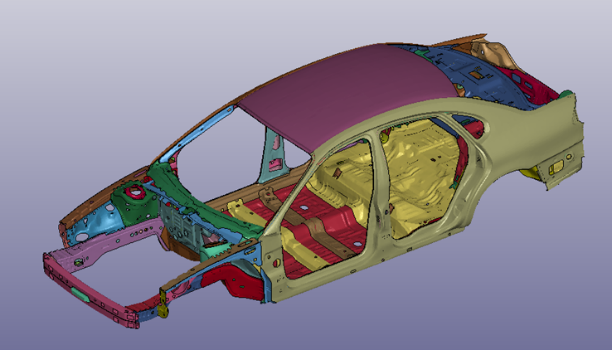
\includegraphics[width=\textwidth]{adhesive_car2.png}

						\vspace{5mm}
						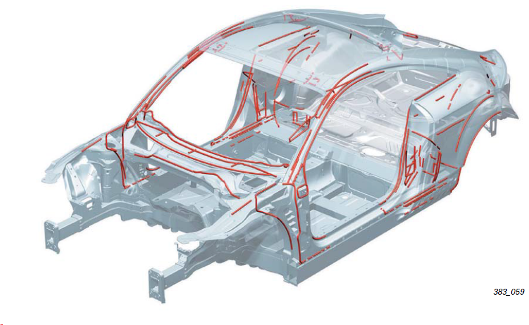
\includegraphics[width=\textwidth]{adhesive_car.png}
				
			\column{.58\linewidth}
			\begin{itemize}
				\item For {Energy conservation}
					\begin{itemize}
						\item weight reduction of cars
						\item \alert{multi-materialization}
						\item \alert{adhesive bonding} technology is a key
					\end{itemize}
				\item durability in long-term use is important
					\begin{itemize}
						\item Especially for alert{fatigue tests}
						\item \alert{reliability of polymer materials is still ambiguous}
					\end{itemize}
			\end{itemize}
			
		\end{columns}

		% 発表ノート
		\note{
			背景から始めましょう。
			\begin{itemize}
				\item 地球温暖化への対策の一環として省エネルギーが注目され、
				\item 車両の軽量化においては、
				\item \alert{マルチマテリアル化が検討}され
				\item \alert{ 接着接合が重要視}されています。
			\end{itemize}
			
			\begin{itemize}
				\item その際に、高分子材料の比強度が高いことはいいのですが、
				\item 疲労破壊に対する耐久性が不明確なことが問題になっています。
			\end{itemize}
		}
\end{frame}


% \subsection{Durability of Rubber}
\begin{frame}
	\frametitle{Mechanical Hysteresis Loss and Fracture Energy}
	\vspace{-1mm}
		% \begin{block}{}
			\begin{columns}[T, onlytextwidth]
				\column{.7\linewidth}
					\begin{itemize}
						\item Mechanical Hysteresis Loss 
							\begin{itemize}
								\item Reduced stress on unloading
								\item Energy dissipation during cycle
								\item \alert{Positive correlation} with fracture energy\footnote{
									\scriptsize{K.A.Grosch, J.A.C.Harwood, A.R.Payne, \\Rub. Chem. Tech., 41, 1157(1968)}
								}
							\end{itemize}
						% \item \alert{Possitive correration} with fracture energy\footnote{
						% 		\scriptsize{K.A.Grosch, J.A.C.Harwood, A.R.Payne, \\Rub. Chem. Tech., 41, 1157(1968)}
						% 	}
						% 	\begin{itemize}
						% 		\item \alert{変形温度}にも強く依存
						% 		\item SBRのガラス転移温度との距離?
						% 	\end{itemize}
						\item The origin of Hysteresis Loss\footnote{
							\scriptsize{A.R.Payne, J.Poly.Sci.:Sympo., 48, 169(1974)}
						}
						\begin{itemize}
							\item \alert{Viscoelastics}
							\color{blue}
							\item Crystallization
							\item Derived by added filler
						\end{itemize}
					\end{itemize}
				\column{.3\linewidth}
				\begin{center}
					\vspace{-2mm}
					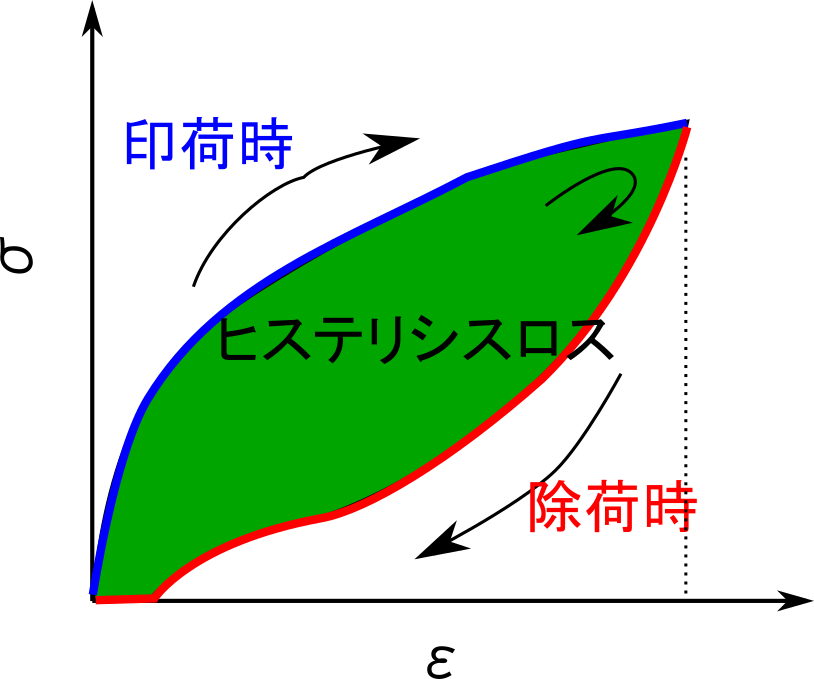
\includegraphics[width=\textwidth]{hysteresis_curve.png}

					\vspace{5mm}
					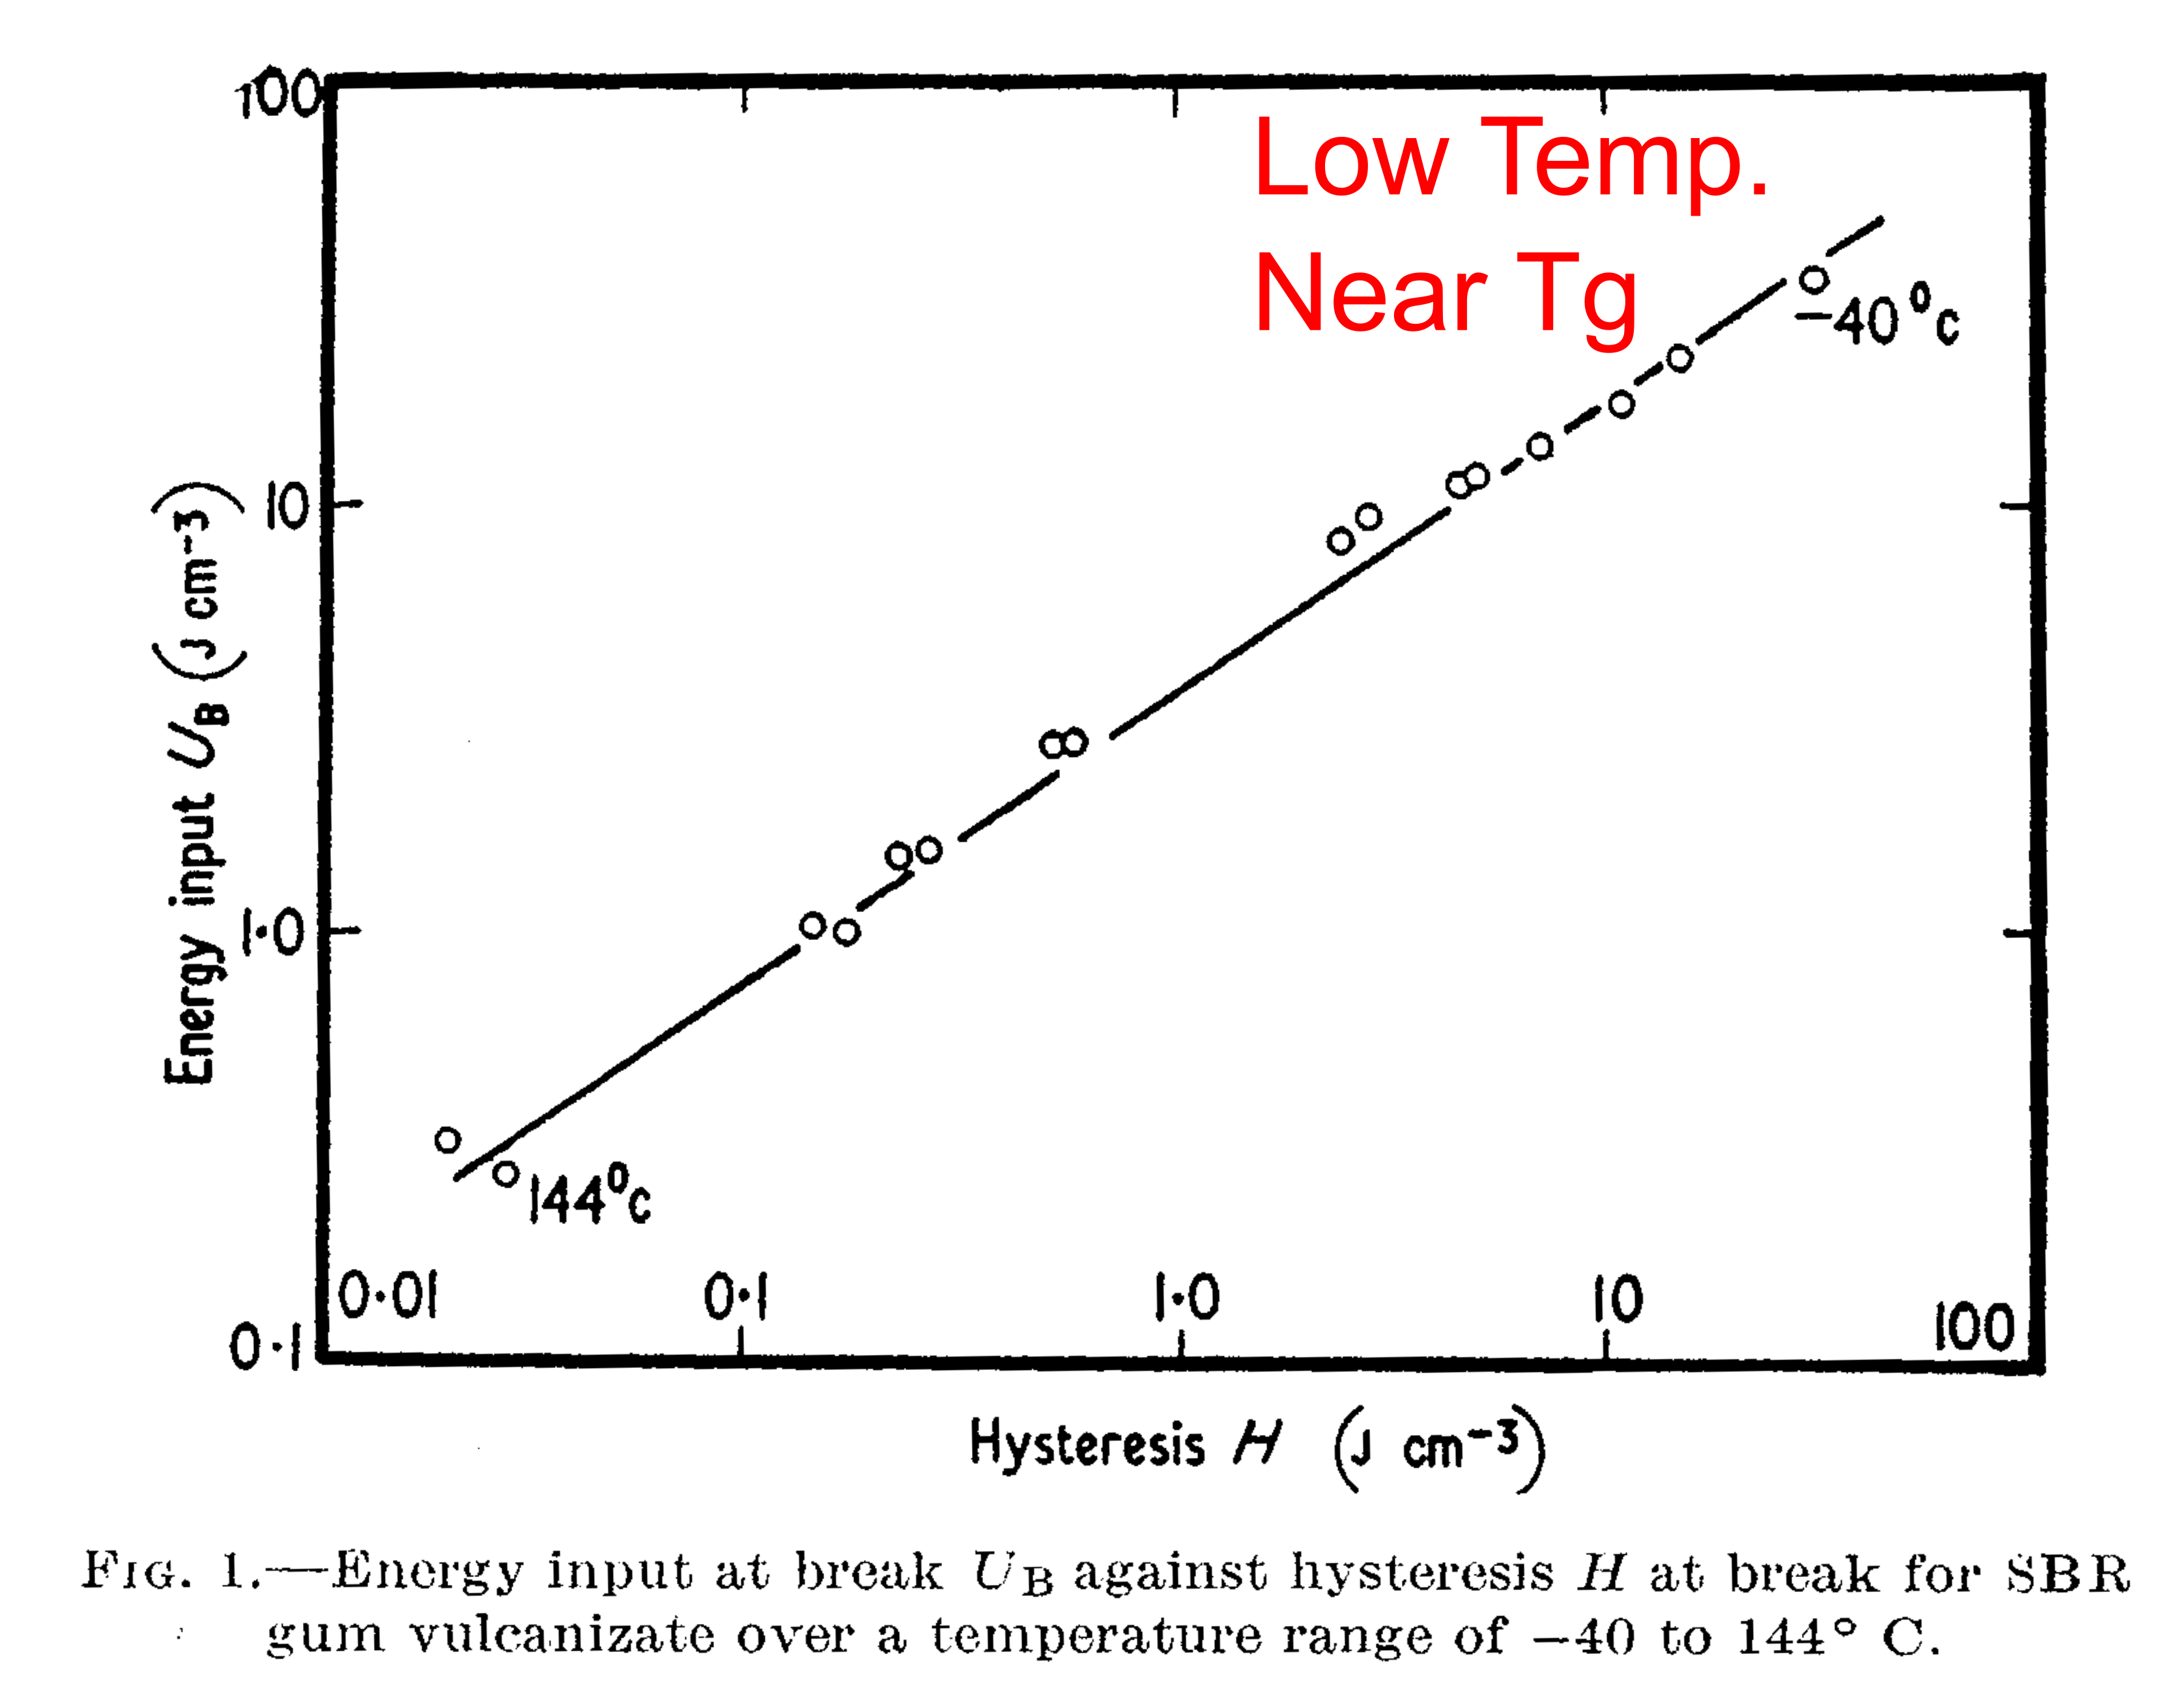
\includegraphics[width=\textwidth]{hyst_break2.png}
				\end{center}
			\end{columns}
		\note{
			\begin{itemize}
				\item \alert{この図に書いた力学的なヒステリシス}は、この緑部分のエネルギー散逸であり、
				\item \alert{破壊エネルギーと相関}することがペインらにより報告されています。
				\item その由来としては、多数考えられますが、
				\item 我々は、この粘弾性起因のものにフォーカスして検討しています。
			\end{itemize}
		}
\end{frame}

\begin{frame}
	\frametitle{Andrews Theory for Rubber Toughness}
	% \vspace{-2mm}
		\begin{exampleblock}{Andrews Theory}
			\begin{columns}[T, onlytextwidth]
				\column{.75\linewidth}
				\begin{itemize}
					\item Focused on \alert{stress field around the crack}\footnote{
						\scriptsize
			{E.H.Andrews, Y.Fukahori, J. of Mat. Sci. 12, 1307 (1977)}
					}
						\begin{itemize}
							\item \textcolor{blue}{Stress Loading zone}
							\item \textcolor{red}{Unloading one}
							\item divided by stress maximum line
						\end{itemize}
					\item On the progress of the crack, 
						\begin{itemize}
							\item \textcolor{green}{stress field is transit}
							\item Hysteresis Loss$\Rightarrow${Energy Dissipation}
							\item The progress of Crack is \alert{Suppressed}
						\end{itemize}
					\item Bigger Hysteresis Loss results in  Higher Toughness.
				\end{itemize}
				\column{.25\linewidth}
					\begin{center}
						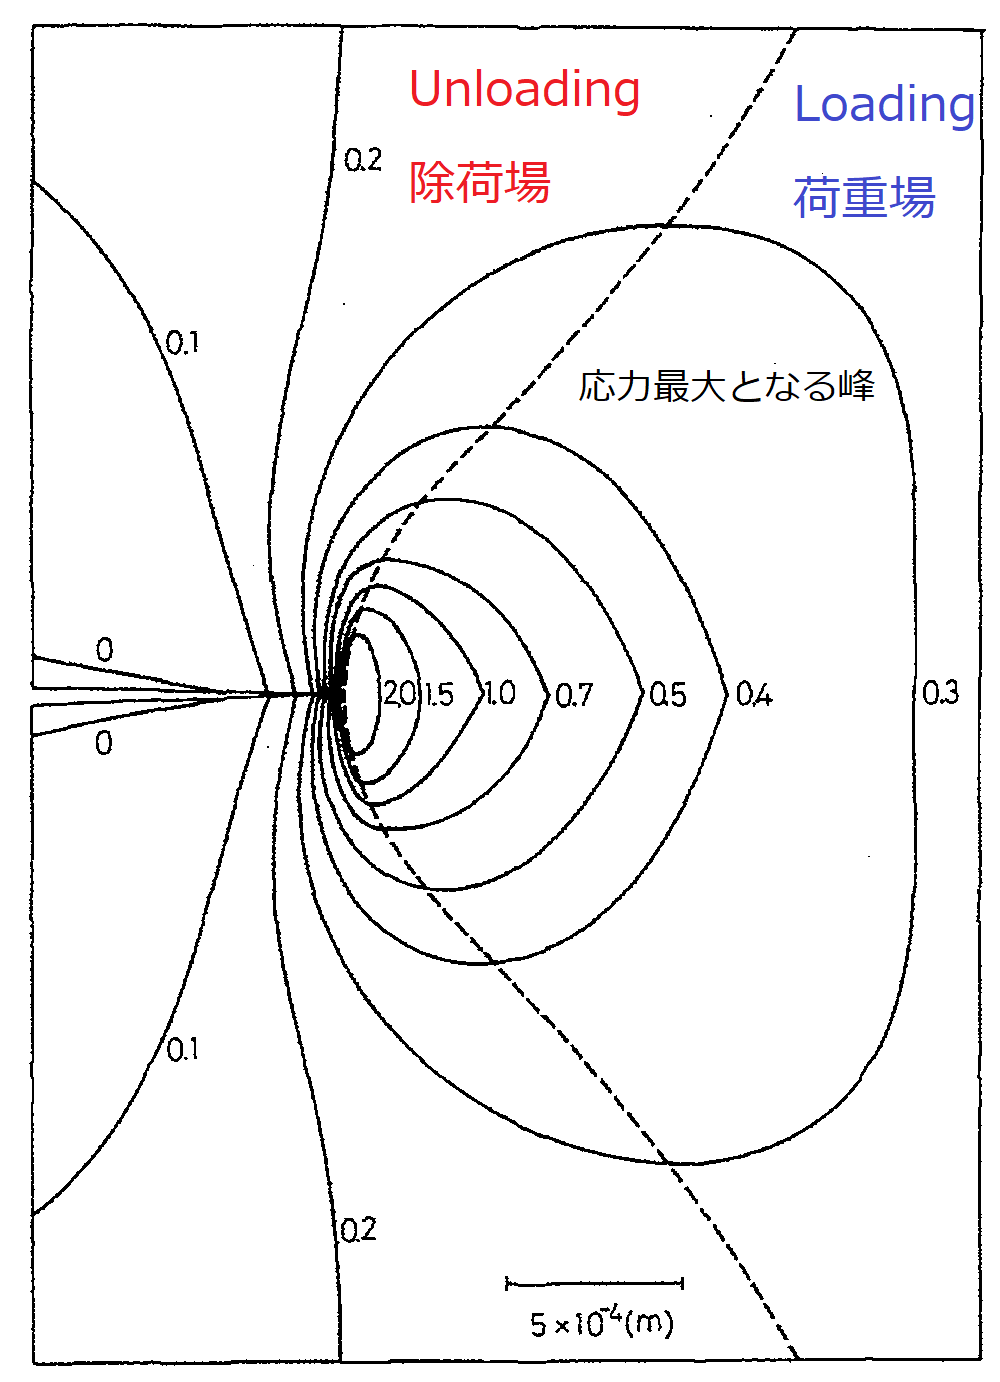
\includegraphics[width=.85\textwidth]{crack.png}
					\end{center}
			\end{columns}
		\end{exampleblock}
		% \vspace{-2mm}
		% \begin{alertblock}{疲労破壊も考慮すると}
		% 	\begin{itemize}
		% 		\item \alert{可逆的}であることが望ましい。\textcolor{blue}{$\neq$ 犠牲結合}
		% 		\item 変形の周期に対応できるように、\alert{回復速度}も重要。
		% 		\item \alert{粘弾性挙動としてのヒステリシスロス$\Leftrightarrow$緩和挙動}
		% 	\end{itemize}
		% \end{alertblock}

		\note{
			\begin{itemize}
				\item ゴム系材料の破壊において、
				\item アンドリューは \alert{クラックチップの先端近傍の応力場に注目}して、
				\item クラック進展に伴い、\alert{荷重場と除荷場が変遷し}、
				\item その際に、\alert{ヒステリシスロスによるエネルギー散逸が存在}すれば、
				\item \alert{クラック進展が抑制}されるという機構を提案しています。
				\item したがって、クラック進展に伴う時間スケールでのヒステリシスロスの大小が、
				\item 破壊耐久性に強い影響を持つということになります。
			\end{itemize}
		}
\end{frame}

\subsection{Theoretical Models for Rubber}
\begin{frame}
    \frametitle{Classical Theory of Rubber Elasticity}
        % \vspace{-2mm}
		% \begin{block}{Free Energy Density of Rubbers against Strain invariant}
		% 	\vspace{-2mm}
		% 	% 非圧縮性条件から第3不変量がおちて、
		% 	\scriptsize
		% 	\begin{align*}
		% 		\dfrac{F}{V} = W 
		% 		% &= \sum_{i,j = 0}^{\infty} C_{ij}(I_1-3)^i(I_2-3)^j \\[-2mm]
		% 		&= C_0 + \underbrace{{\color{green}C_1(I_1-3)} + {\color{red}C_2(I_2-3)}}_{\color{red}Mooney-Rivlin Model} + \sum_{i,j = 1}^{\infty} C_{ij}(I_1-3)^i(I_2-3)^j
		% 	\end{align*}  
		% \end{block}
		% \vspace{-5mm}
		\begin{columns}[T, onlytextwidth]
			\column{.48\linewidth}
				\begin{exampleblock}{Neo-Hookean Model}
					\vspace{-2mm}
					% 第1不変量のみを対象
						\scriptsize
						\begin{align*}
							&W = C_1 (I_1-3) \\
							&\text{against Uniaxial elongation} \\
							&\sigma_{nom} = 2 C_1\left(\lambda - \dfrac{1}{\lambda^2}\right) = G \left(\lambda - \dfrac{1}{\lambda^2}\right)
						\end{align*}
				\end{exampleblock}
			\column{.48\linewidth}
				\begin{alertblock}{Mooney-Rivlin Model}
					\vspace{-2mm}
					% 高次の項をおとす
					\scriptsize
					\begin{align*}
						&W = C_1 (I_1-3) + C_2(I_2-3) \\
						&\text{against Uniaxial elongation} \\
						&\sigma_{nom} = 2 \left(C_1 + C_2\dfrac{1}{\lambda} \right) \left(\lambda - \dfrac{1}{\lambda^2}\right)
					\end{align*}
				\end{alertblock}
		\end{columns}
		% \vspace{-1mm}
		\begin{block}{With or without Junction Poinits fluctuation}
			\vspace{1mm}
			\begin{columns}[T, onlytextwidth]
				\column{.48\linewidth}
				\small
				\color{blue}{Affine Network Model
				\footnote{
					\tiny{P.J. Flory, Principles of Polymer Chemistry, (1953)}
				}
				}
				\vspace{-2mm}
				\scriptsize
				\begin{align*}
					% &\text{Affine Network Model}\\
					&G_{affine} = \nu k_B T  \\
					&\text{$\nu$: Number density of strands in the system}
				\end{align*}
				\column{.48\linewidth}
				\small
				\color{magenta}{Phantom Network Model
				\footnote{
					\tiny{H.M. James, E.J. Guth, Chem. Phys., 21, 6, 1039 (1953)}
				}
				}
				\vspace{-2mm}
				\scriptsize
				\begin{align*}
					% &\text{Phantom Network Model}\\
					&G_{phantom} = \nu k_B T \left(1 - \dfrac{2}{f}\right) \\
					&\text{$f$: Functionality of Junction Points}
				\end{align*}
				\normalsize
			\end{columns}
		\end{block}

		\note{
			さて、少し話題を変えて、ゴム弾性についての古典的な取り扱いを振り返ってみます。
			\begin{itemize}
				\item 最も単純化した取り扱いとして、結節点がマクロな変形と相似となる Affine Network model が提案された後、
				\item 結節点のゆらぎを考慮した Phantom Network Model が提案されています。
				\item この際、結節点の分岐度に応じて、弾性率が低減します。
			\end{itemize}
		}
\end{frame}

\begin{frame}
	\frametitle{Constraint Factors for Junction Points and Strands}
		\vspace{-2mm}
		\begin{alertblock}{Vicinity of Junction Point}
			\begin{columns}[totalwidth=1\textwidth]
				\column{.75\textwidth}
				\vspace{-3mm}
				\begin{itemize}
					\item Junction points are surrounded by many of \alert{adjacent strands(x in fig.).}
					\item Fluctuation of junctions are \alert{suppressed}. 
				\end{itemize}
				\column{.22\textwidth}
				\centering
				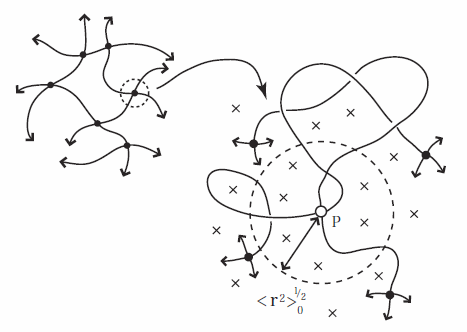
\includegraphics[width=\textwidth]{JP_vicinity.png}
			\end{columns}
		\end{alertblock}
		\vspace{-1mm}
		\begin{block}{Effect of other strands (Combination of $G_c$ and $G_e$)}
			\only<1>{
				\begin{itemize}
					\item Suppress the fluctuation of Junction Point
					\begin{itemize}
						\item Deviate from Phantom Network Model and higher $G_c$
					\end{itemize}
					\item Strands Entangles each other
					\begin{itemize}
						\item Works as a Junction Point
						\item Generate additional $G_e$
					\end{itemize}
				\end{itemize}
				Storage modulus $G$ is \alert{combination of $G_c$ and $G_e$}
			}
			\only<2>{
				\begin{columns}[totalwidth=1\textwidth]
					\column{.65\textwidth}
					\begin{itemize}
						\item Constrained Junction Model
						\begin{itemize}
							\item  $G$ approaches to $G_c$.\footnote{\tiny{P.J.Flory, J.Chem.Phys., 66, 12, 5720 (1977)}}
						\end{itemize}
						\item Topological relationships
						\begin{itemize}
							\item Contribution of entanglement.\footnote{\tiny{D.S.Pearson and W.Graessley, Macromol., 11, 3, 528 (1978)}}
							\vspace{-2mm}
							\scriptsize
							\begin{align*}
								G_e = T_e G_N^0
							\end{align*}
						\end{itemize}
					\end{itemize}
					\column{.25\textwidth}
					\vspace{-2mm}
					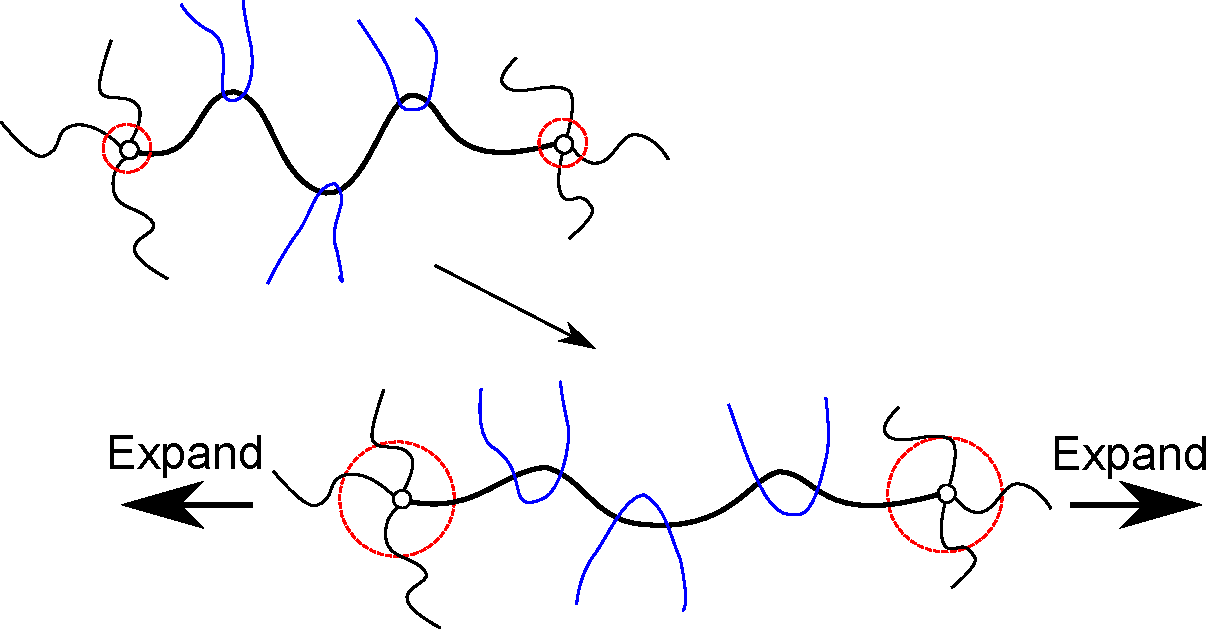
\includegraphics[width=\textwidth]{Constrained_Juntion.pdf}
	
					\vspace{3mm}
					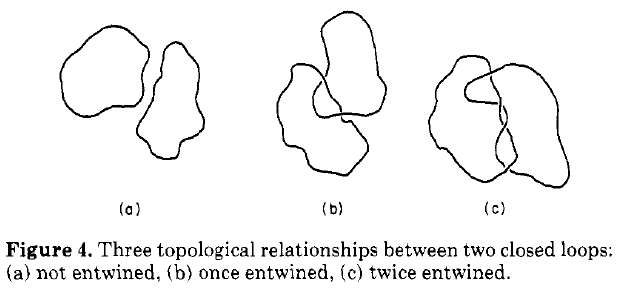
\includegraphics[width=\textwidth]{topological_effect_ring.png}
				\end{columns}
			}

			\note{
				\begin{itemize}
					\item 結節点の近傍では、
					\begin{itemize}
						\item Junction points は \alert{近接するストランド} に囲まれ、
						\item ゆらぎは \alert{抑制されます}. 
					\end{itemize}
					\item その効果は2つあり、
					\begin{itemize}
						\item ゆらぎを抑制し、Affineモデルへと近づき、
						\item 他の効果としては、空間的にトラップされた絡み合いが付加的な弾性率 $G_e$ を生じます。
						\item その結果として、弾性率は \alert{combination of $G_c$ and $G_e$}
					\end{itemize}
					\item \textcolor{red}{(CLICK)}
					\item この問題に対して、2つのアプローチがあり、
					\begin{itemize}
						\item その一つは Constrained Junction model, 
						\item on the uniaxial deformation, constraints are released and $G$ approaches to $G_c$
						\item もう一つが、トラップ土エンタングルメントの検討です。
					\end{itemize}
				\end{itemize}
			}
		\end{block}

			
\end{frame}

\setcounter{footnote}{0}
\begin{frame}
	\frametitle{Recent approach for Constraints (Entanglements)}
	\vspace{-2mm}
		\begin{itemize}
			\item Diffused-Constraint Model
			\begin{itemize}
				\item Confining potential affect all points along the chain.\footnote{\tiny{A. Kloczkowski, J.E. Mark, B. Erman, Macromol., 28, 5089 (1995)}}
			\end{itemize}
			\item Nonaffine Tube Model
			\begin{itemize}
				\item Improved model of "Edwards' Tube Model".\footnote{\tiny{M. Rubinstein, S. Panyukov, Macromol., 30, 25, 8036 (1997)}}
			\end{itemize}
			\item \alert<2>{Slip-tube Model}
			\begin{itemize}
				\item A pairwise interaction of chains is introduced.\footnote{\tiny{M. Rubinstein, S. Panyukov, Macromol., 35, 6670 (2002)}}
			\end{itemize}
		\end{itemize}

		\vspace{1mm}
		\centering
		\visible<2>{
			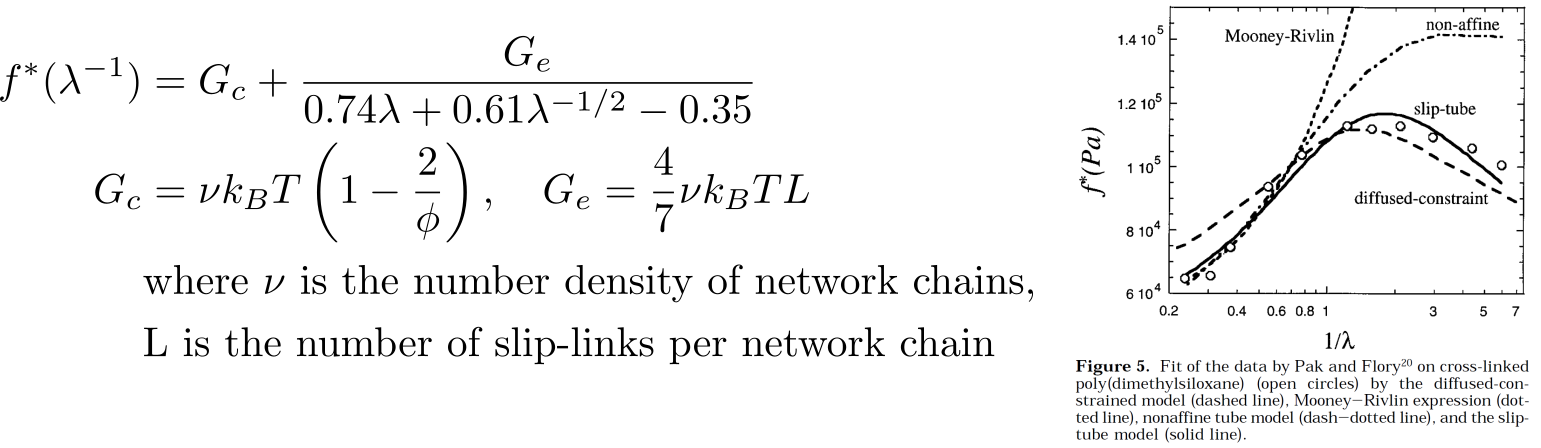
\includegraphics[width=.9\textwidth]{rubinstein_4.png}
		}
		\note{
			\begin{itemize}
				\item 近代的な検討はこの3つであり、
				\item どれも、Phantom Network Model をベースにしたものです。
				\item Rubinstein's の Slip-tube model は、
				\item \textcolor{red}{(Point and CLICK)}
				\item 比較的単純に Gc と Ge を分割しており、
				\item その影響が変形とともに減少する過程を記述します。
			\end{itemize}
		}
\end{frame}

\subsection{Objectives}
\setcounter{footnote}{0}
\begin{frame}
	\frametitle{Random Networks as a key for PNM}
		\begin{columns}[c, onlytextwidth]
			\column{.72\linewidth}
			\begin{itemize}
				\item Introduction of \alert{Random Connectivity}.
					\item \alert{Criteria for PNM} is fulfilled\footnote{
								\scriptsize{P. J. Flory, Proc. R. Soc. London. A, 351, 351 (1976)}
						}.
					\begin{itemize}
						\item the mean values $\bar{\bm{r}}$ of strands are \alert{fluctuate}
						\item fluctuations $\Delta \bm{r} = \bm{r} - \bar{\bm{r}}$ are \alert{Gaussian}
						\item the mean-square fluctuations \alert{depend only on structure}
					\end{itemize}
					% \end{itemize}
				\item Previous Work for Random Network
				\begin{itemize}
					\item \alert{Random endcrosslink for telechelics}\footnote{
						\scriptsize{G.S. Grest, et.al., Non-Cryst. Solids, 274, 139 (2000)}
						}
					\item \alert{Primitive Chain Network Simulation}\footnote{
						\scriptsize{Y. Masubuchi, Nihon Reoroji Gakkaishi, 49, 2, 73 (2021)}
					}
				\end{itemize}
			\end{itemize}
			\column{.26\linewidth}
				\centering
					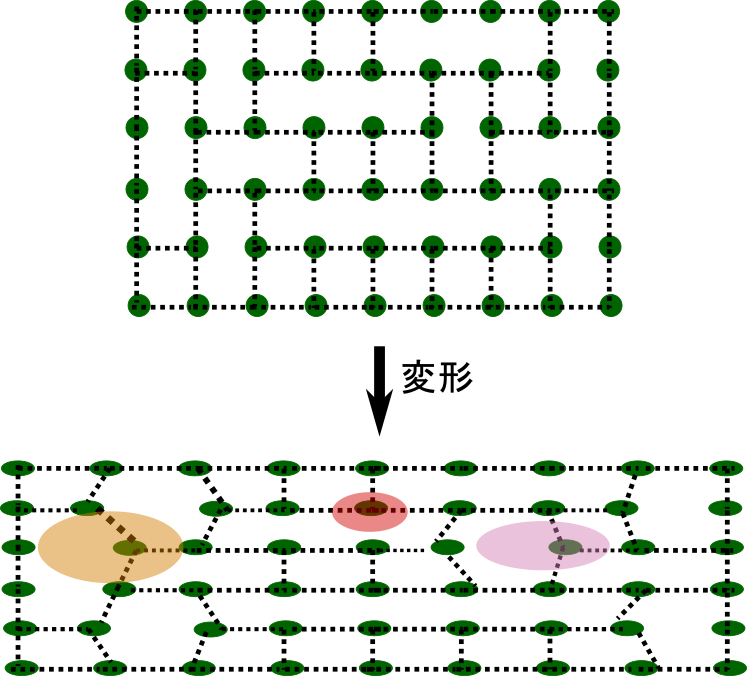
\includegraphics[width=\textwidth]{random_NW.png}
		\end{columns}

		\note{
			\begin{itemize}
				\item ランダムな接続性が Phantom Network model のキーとなることが知られており、
				\item \textcolor{red}{(POINT)}
				\item ここに示したような、クライテリアを充足するようです。
				\item \textcolor{red}{(POINT)}
				\item この2つの先行研究がシミュレーションとして知られていますが、
			\end{itemize}
		}
\end{frame}

\begin{frame}
	\frametitle{Objectives}

	\begin{itemize}
		\item Recent approach for rubber elasticity models are based on Phantom Network Model.
		\item Introducing random connectivity, MD simulation studies were carried out.
		\item To investigate the criteria for Phantom Network Model, Two model chains are used.
		\begin{enumerate}
			\item Employing phantom chain, basics for PNM is examined.
			\item Changing the chain to KG Chain, constraints effects are investigated.
			\begin{itemize}
				\item Excluded Volume Effect
				\item No mutual crossing of Strands
			\end{itemize}
		\end{enumerate}
	\end{itemize}

	\note{
		本検討のオブジェクトについて説明します。
		\begin{itemize}
			\item ゴム弾性に対する現代的なアプローチは、\alert{Phantom Network Model}をベースにしたものとなっています。
			\item そこで、我々は、
			\item ランダムな接続性を導入したネットワークモデルのMDシミュレーションでのPhantom Network Modelの検討を行ってきました。
			\item 本日は、以下の二点についてまとめた結果をお話します。
			\begin{enumerate}
				\item ストランドとして、す抜け鎖であるファントム鎖を用いてPhantom Network Modelとの整合性を確認
				\item ストランドを \alert{KG Chain}に変更して、その差異を検討
				\begin{itemize}
					\item KG Chainは
					\item 排除体積効果があり、
					\item ストランドの相互すり抜けが抑制
				\end{itemize}
			\end{enumerate}
		\end{itemize}
	}
\end{frame}

\section{Simulation}
\subsection{Generation Recipe of Random Networks}

\begin{frame}
	\frametitle{Generation of Initial Structure of Random Networks}
	\begin{enumerate}
		\item 8-Chain Model is used as starting structure in \alert{Real space}.
			\begin{itemize}
				\item Randomly selected edge is removed until desired functionality.
				\item Topological model is generated. 
			\end{itemize}
		\item Randomness is introduced in \alert{topological space}.
			\begin{itemize}
				\item By \alert{edge exchange}, random connectivity is introduced for each node.
			\end{itemize}	
		\item Corresponding real space structure is generated.
		\item According to e2e distance of strand, system size and multiplicity are set.
	\end{enumerate}

	\vspace{-1mm}
	\begin{columns}[T, onlytextwidth]
		\column{.33\linewidth}
			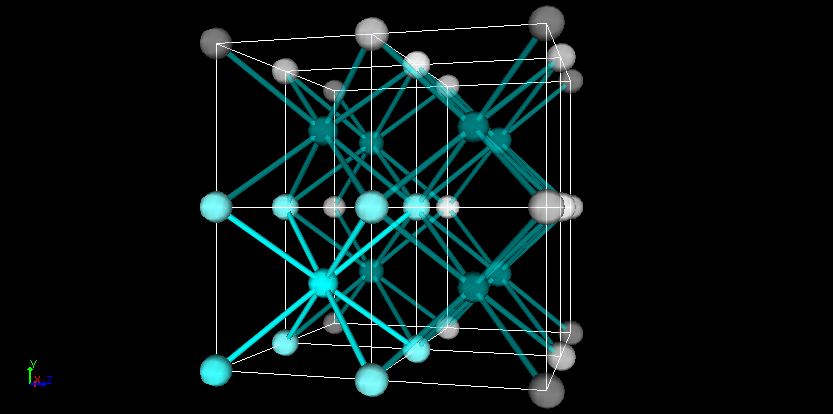
\includegraphics[width=\textwidth]{8_per.png}
		\column{.33\linewidth}
			\vspace{-5mm}
			\begin{center}
				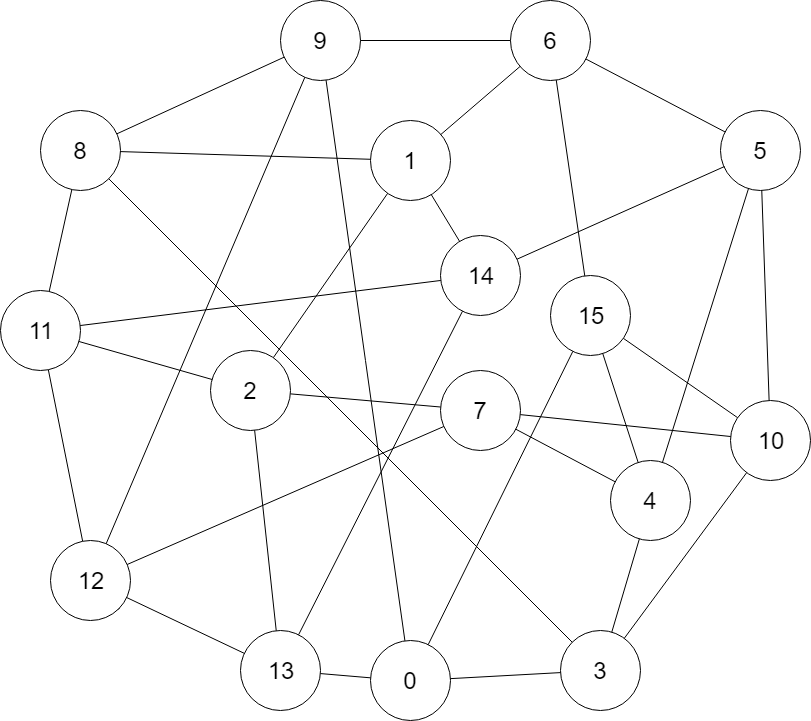
\includegraphics[width=.6\textwidth]{Network.png}
			\end{center}
		\column{.33\linewidth}
			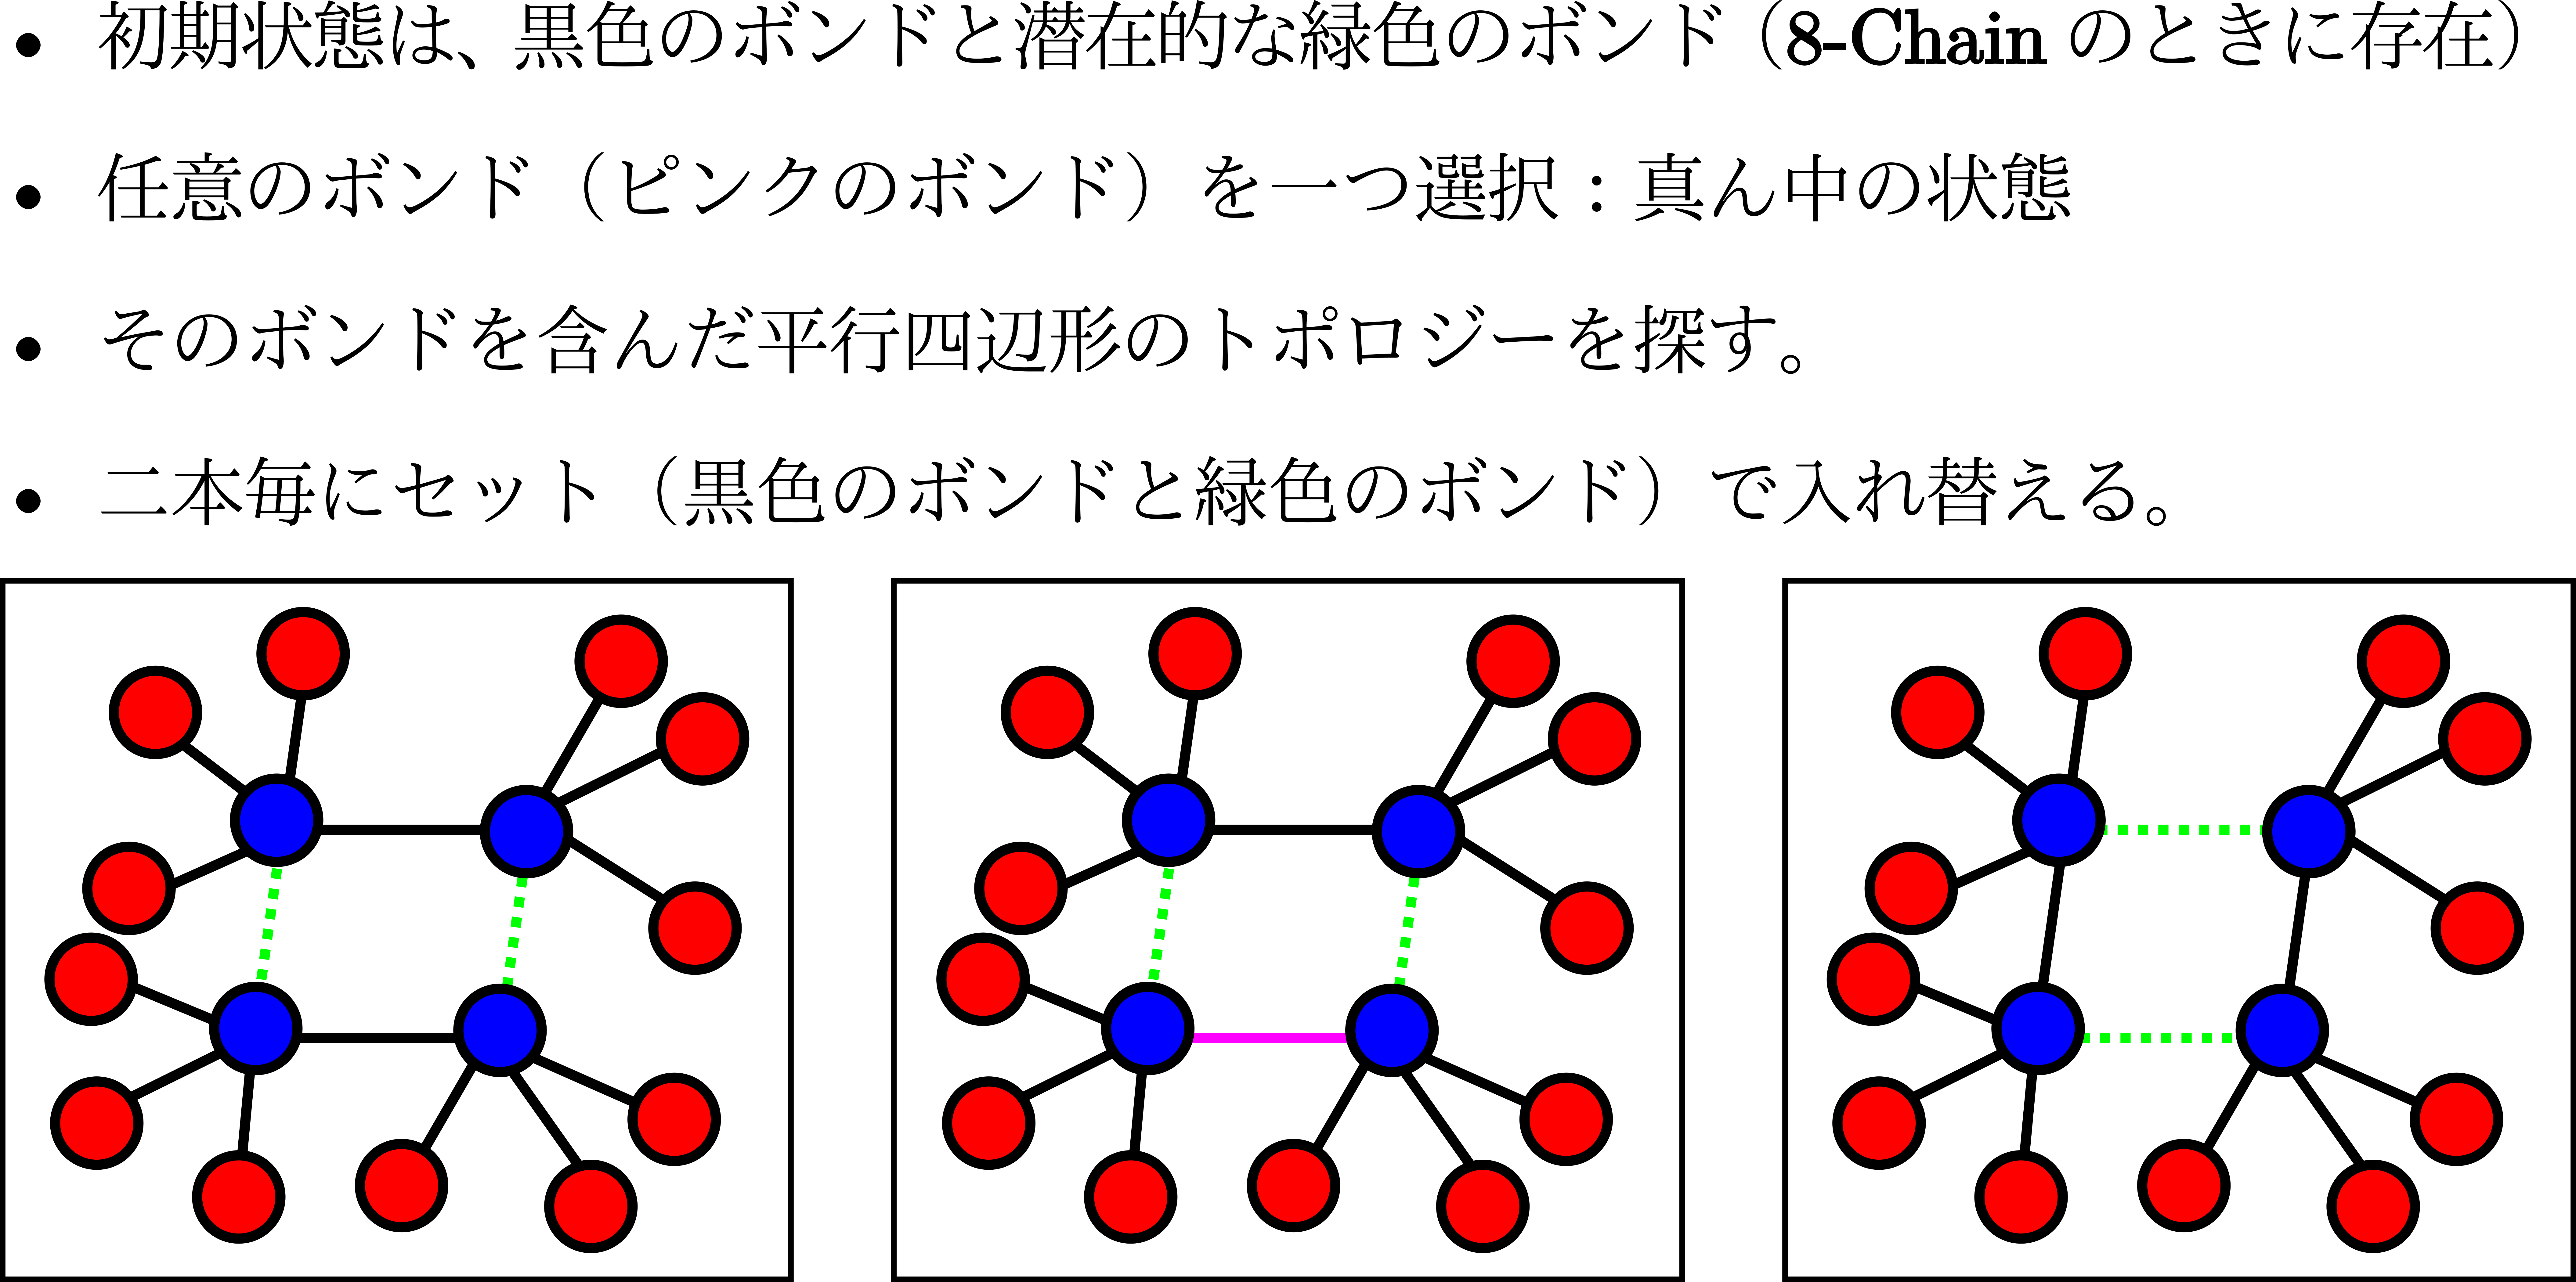
\includegraphics[width=\textwidth]{bond_exchg.png}
	\end{columns}
	
	\note{
		ランダムなネットワークの初期構造の作成を簡単に説明します。
		\begin{itemize}
			\item 最初に実空間で 8-Chain Model を用います。
				\begin{itemize}
					\item ランダムに選択されたストランドを所望の分岐度になるまで消去し、
					\item この真ん中に示した位相空間でのトポロジカルモデルとします。 
				\end{itemize}
			\item \alert{位相空間において}、ネットワークの接続性を確認しながら、 \alert{ストランド交換を繰り返す。}	
			\item 十分に交換を行った後に、実空間でのモデルへと戻します。
			\item ストランドの末端間距離に対応した長さとなるようにシステムサイズを決め、
			セグメント密度が $\rho = 0.85$ となるように多重度も決めます。
		\end{itemize}
	}
\end{frame}

\subsection{Phantom and KG Chains as Strands}
\begin{frame}
	\frametitle{Phantom and KG Chains as Strands}
	\begin{itemize}
		\item Phantom Chain:
		\begin{itemize}
			\item No Excluded Volume is set (no segmental interaction).
			\item "Force Cap LJ" is set as Angle Potential to enumerate e2e length of KG Chains.
			\item Harmonic bond(k=1000)
		\end{itemize}
		\item KG Chain:
		\begin{itemize}
			\item Excluded Volume is set by Repulsive LJ Potential.
			\item Bond Potential is set to FENE.
			\item Because of above two potentials, No Chain crossing will occur.
		\end{itemize}
	\end{itemize}

	\note{
		\begin{itemize}
			\item Phantom and KG Chains の条件をまとめました。
			\item 今回のシミュレーションで重要なポイントは、
			\item ファントム鎖において、
			\item "Force Cap LJ" という仕組みでストランドのセグメント間に 1,3 相互作用を導入して、
			\item セグメント間のアングルがKG鎖と同等となるように設定し、末端間距離も整合するようにしたことです。
			\item KG鎖においては、通常の斥力系の条件を用いています。
		\end{itemize}
	}
\end{frame}


\subsection{Simulation Conditions}
\begin{frame}
    \frametitle{Reluxation of Initial Structure in KG Network}
        \vspace{-2mm}
		\begin{block}{KG Network: KG chain as strand}
			\begin{itemize}
				\item \alert{Relaxation of initial structure} is important.
					\fontsize{6pt}{0pt}
					\begin{align*}
						&U_{KG}(r) = 
						\begin{cases}
						U_{nonbond} = U_{LJ} \;\text{where } r_c = 2^{(1/6)}\sigma \\
						U_{bond} = U_{LJ} + U_{FENE}
						\end{cases} 
					\end{align*}
			\end{itemize}
		\end{block}
		\vspace{-3mm}
		\begin{columns}[T, onlytextwidth]
			\column{.66\linewidth}
				\begin{exampleblock}{Initial Structure Relaxation}
					\begin{itemize}
						\item According method of Auhl\footnote{
							\scriptsize{R. Auhl et al. J. of Chem. Phys., 119, 12718 (2003)}
						}
						\begin{itemize}
							\item Using force-capped-LJ pot.
							\item relaxed by Slow Push Off
						\end{itemize}
					\end{itemize}
					\fontsize{6pt}{0pt}
					\begin{align*}
						&U_{FCLJ}(r) = 
						\begin{cases}
						(r-r_{fc})*U_{LJ}^{\prime}(r_{fc}) + U_{LJ}(r_{fc}) \; &r< r_{fc} \\
						U_{LJ}   \;\;\;\;\;\;\; &r \geq r_{fc}
						\end{cases} 
					\end{align*}
				\end{exampleblock}
			\column{.32\linewidth}
				\vspace{2mm}
				\begin{center}
					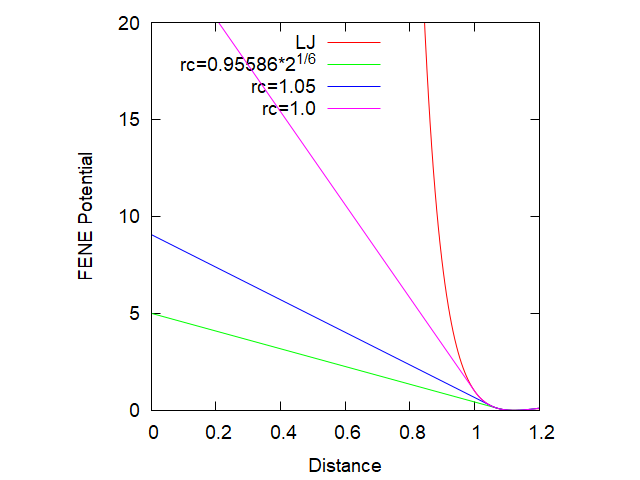
\includegraphics[width=1.2\textwidth]{Ev_fcLJ.png}
				\end{center}
				\vspace{-3mm}
				\scriptsize
				\begin{itemize}
					\item force-capped-LJ Pot.
					\item gradually entangled
				\end{itemize}
		\end{columns}

		\note{
			\begin{itemize}
				\item 相互の鎖のすり抜けの生じないKG鎖では、初期構造の生成が重要です。
				\item ここに示した force-capped-LJ pot.により、
				\item 少しずつ鎖のすり抜け度合いを強めて適切な初期構造を。
			\end{itemize}
		}
\end{frame}

\section{Results}
\subsection{Networks with Phantom Chains}

\begin{frame}
	\frametitle{
		Strand length Effect for Phantom Chain NW
	}
	\begin{itemize}
		\item Strand-length is varied \alert{from 36 to 48 for f=4}
		\item System size is reduced to keep $\rho = 0.85$
	\end{itemize}

	\begin{figure}[htb]
		\centering
			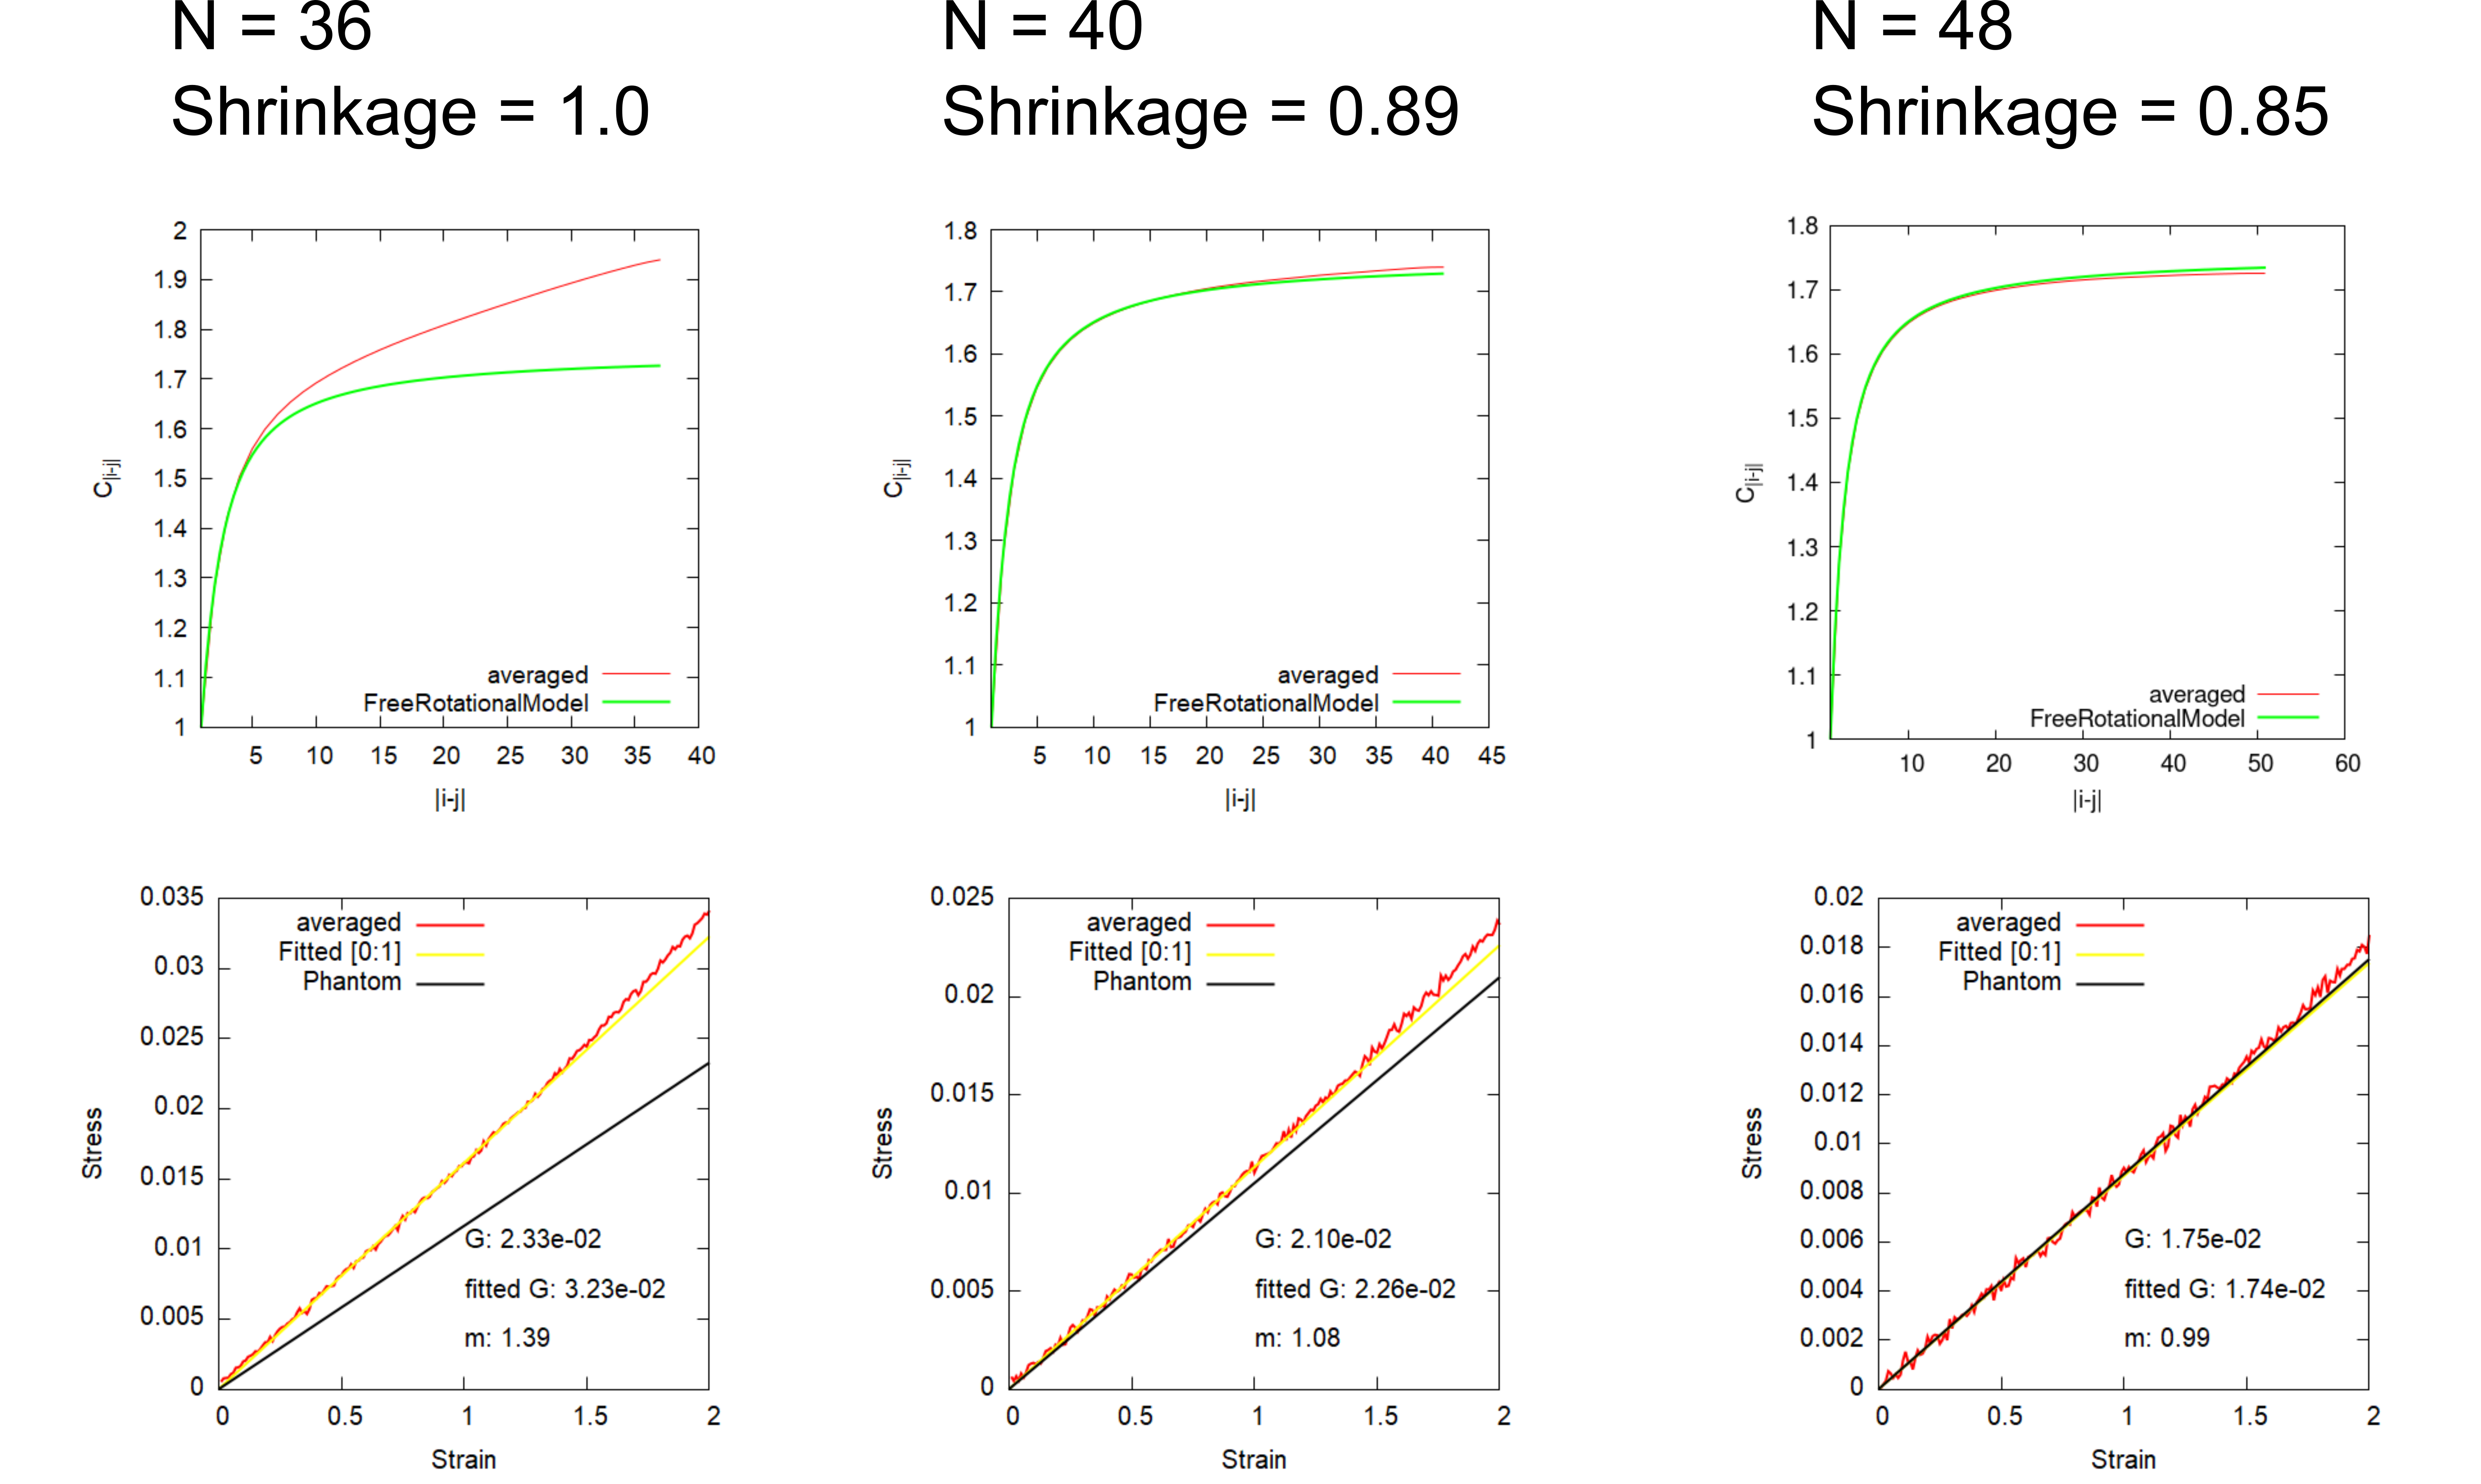
\includegraphics[width=.8\textwidth]{N36_N40_N48.png}

			\scriptsize{Strand Length Comparison for Shear Stress}
	\end{figure}

	\note{
		\begin{itemize}
			\item N=36が先ほど示した条件でストランドが自然長になる条件なんですが、
			\item 鎖に沿ったセグメント間距離を見ると随分伸長されていて、
			\item ズリせん断印加時の応力もPNMよりも高くなっていた。
			\item ストランドのセグメント数を増加し、かつ、系を収縮することで
			\item 応力がPNMの予想するものと一致した。
			\item \textcolor{red}{(POINT N=48)}
			\item このことから、ストランド長が適切でなければ結節点のゆらぎを抑制し、その結果PNMから乖離していくと推定できた。
		\end{itemize}
	}
\end{frame}

\begin{frame}
	\frametitle{
		Comparison of Functionality (f = 3, 4, 6)
	}

	\begin{figure}[htb]
		\centering
			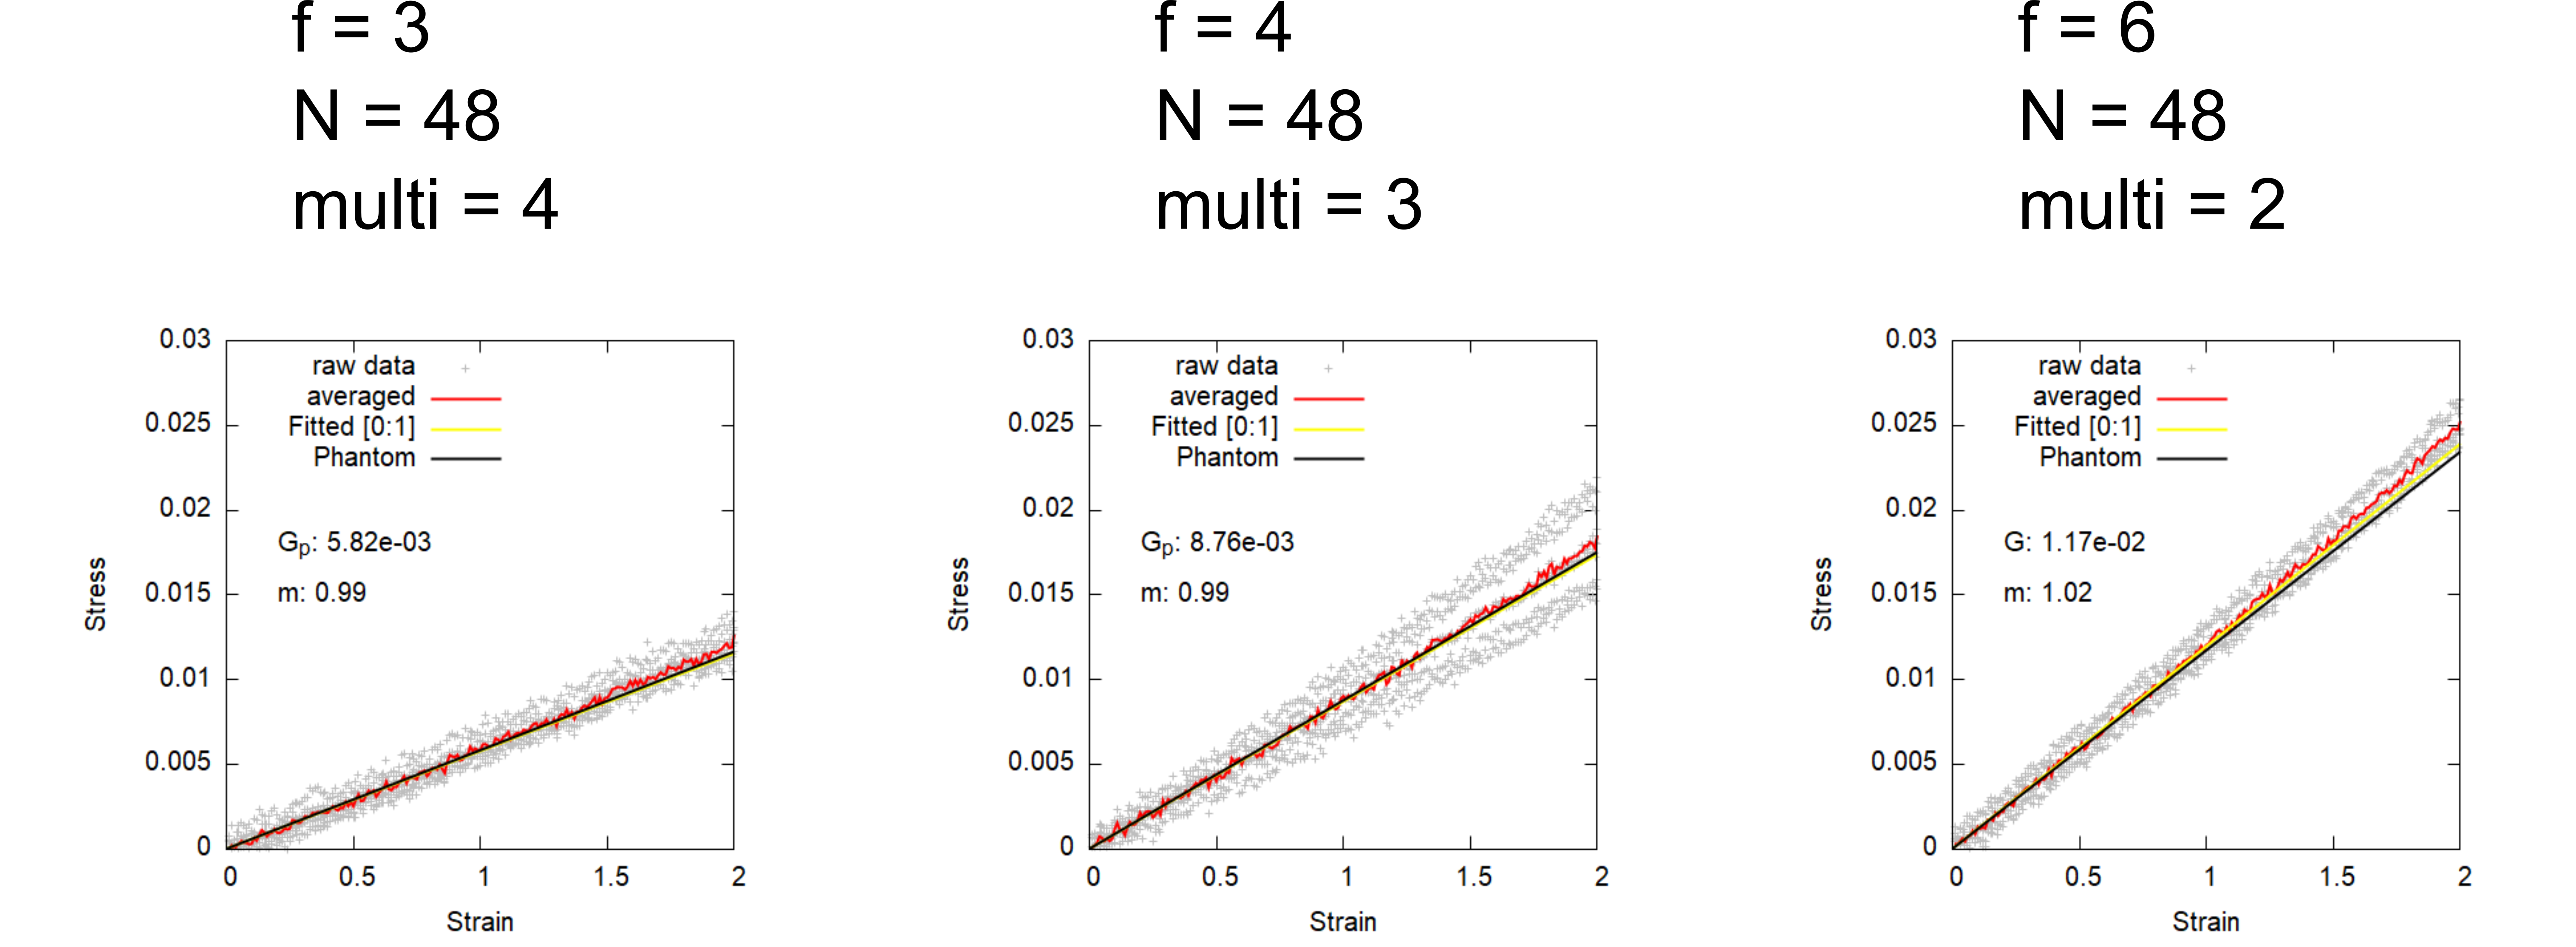
\includegraphics[width=\textwidth]{compare_346.png}

			% \scriptsize{Comparison of Functionality (f = 3, 4, 6)}
	\end{figure}

	\note{
		\begin{itemize}
			\item 適正なストランド帳である N=48 では、
			\item 分岐数の影響もきれいにPNMに合致していた。
			\item \textcolor{red}{(POINT all)}
		\end{itemize}
	}
\end{frame}

\subsection{KG Chain Networks}
\begin{frame}
	\frametitle{Mechanical Responce for KG Chains(f=4, N=48)}
	\vspace{-3mm}
	\begin{alertblock}{4-Chain Random Network with KG Chain}
		\begin{itemize}
			\item Excluded Volume Effect by non-bonding LJ Potential.
			\item No strands mutual crossing by FENE bond.
		\end{itemize}
	\end{alertblock}
	\vspace{-4mm}
	\begin{columns}[T, onlytextwidth]
		\column{.48\linewidth}
			\begin{block}{Phantom Chain}
				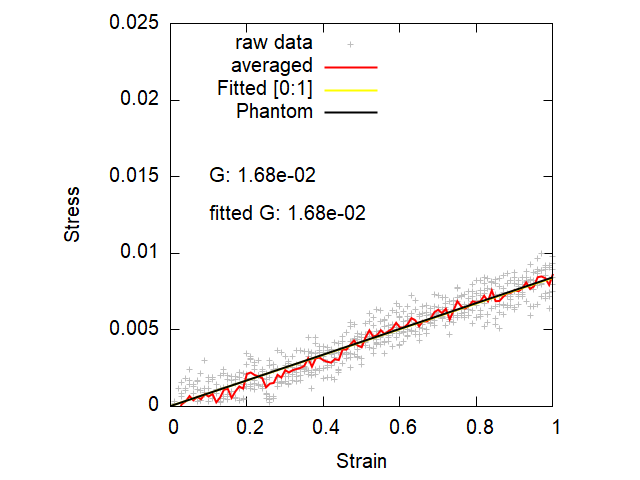
\includegraphics[width=\textwidth]{4chain_N50_PNM_shear.png}
			\end{block}
			
		\column{.48\linewidth}
			\begin{block}{KG Chain}
				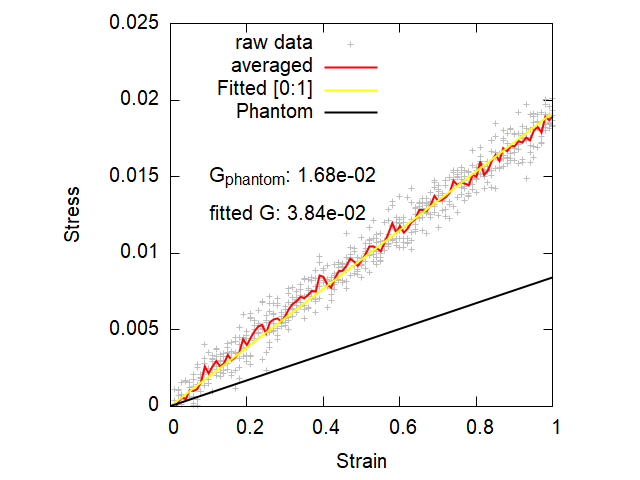
\includegraphics[width=\textwidth]{4chain_N50_shear.png}
			\end{block}
	\end{columns}

	\note{
		\begin{itemize}
			\item ファントムネットワークの結果に基づいて、同一のストランド長でKG鎖の検討を行いました。
			\item その結果、モデュラスは高くなることが確認できました。
			\item \textcolor{red}{(POINT)}
		\end{itemize}
	}
\end{frame}

% \begin{frame}
%     \frametitle{Analysis of Entanglements in Network: Z1-code}
%         \vspace{-2mm}
%         \begin{columns}[onlytextwidth][c]
%             \column{.3\linewidth}
%                 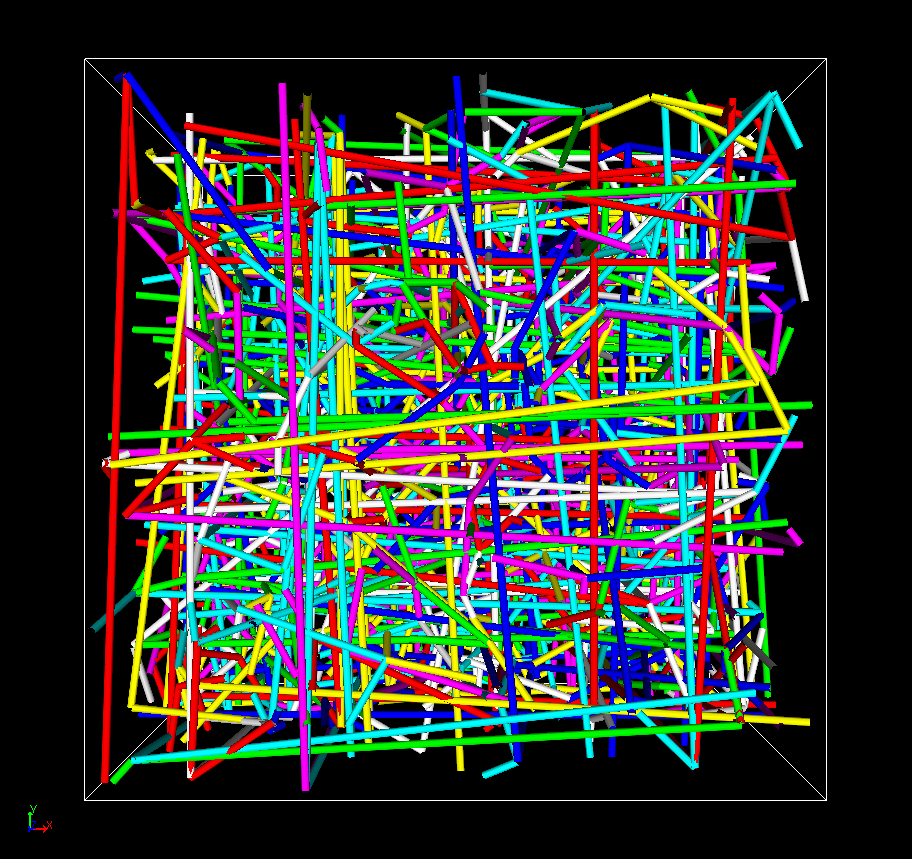
\includegraphics[width=\textwidth]{z_cord_4Chain.png}
% 				% \caption{Entanglements by Z-1 Code}
				
%             \column{.6\linewidth}
%             \begin{block}{Comparison with Homopolymer Melt}
%                 \begin{itemize}
%                     \item Z is number of entanglements per chain
%                     % \item 今回のネットワークは、\\ホモポリマーと同等
%                 \end{itemize}
%                 \scriptsize
%                 \begin{center}
%                     \begin{tabular}{c||c|c} \hline
%                         &Homo & 4 Chain NW \\ \hline \hline
%                         Segments& 50& 48 \\ \hline
%                         Chains & 200& 768 \\ \hline
%                         Entanglements& 204& 800\\ \hline
%                         Entangled Chains&134&557 \\ \hline
%                         \alert{$<Z>_{Z1}$}&\alert{1.02}& \alert{1.04}\\ \hline
%                     \end{tabular}
%                 \end{center}
%             \end{block}
%         \end{columns}
%     \begin{alertblock}{Z1-code?}
%         \begin{itemize}
%             \item Z1-code is an algorism to visualize and count entanglements\footnote{
%                 M. Kröger, Comput. Phys. Commun. 168, 209 (2005)
%             }
%         \end{itemize}
%     \end{alertblock}
% 	\note{
% 		\begin{itemize}
% 			\item この弾性率増加の原因を明確にするため、絡み合いを表すZを見てみました。
% 			\item Zは同じ長さのストランドの直鎖ポリマーとほぼ同一であり適正な初期化も確認できました。
% 			\item \textcolor{red}{(POINT left two)}
% 			\item 1.02 and 1.04
% 		\end{itemize}
% 	}
% \end{frame}

\begin{frame}
    \frametitle{Reduced Entanglements by NPT Model}
        % \vspace{-3mm}
		\begin{columns}[c, onlytextwidth]
            \column{.4\linewidth}
                \footnotesize
				\begin{itemize}
					\item 4-Chain-\alert{NPT}\\
					$<Z>_{Z1}$ = 0.36

					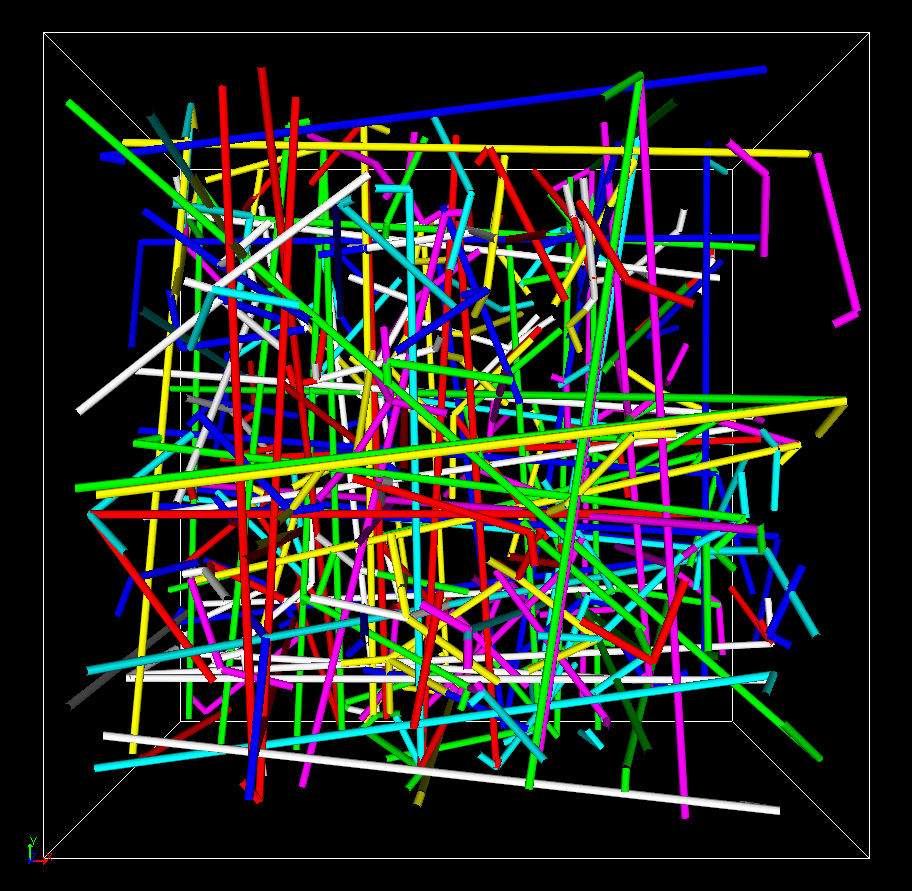
\includegraphics[width=.62\textwidth]{z_cord_NPT_4Chain.png}
					\item 4-Chain-NVT\\
					$<Z>_{Z1}$ = 1,04

					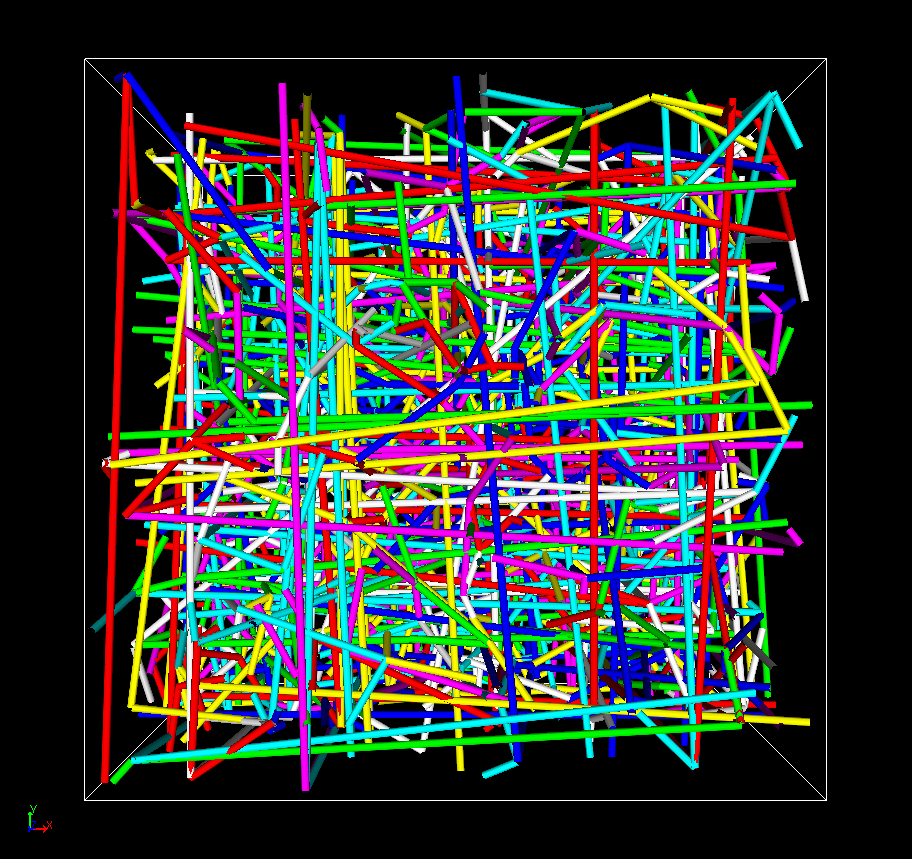
\includegraphics[width=.62\textwidth]{z_cord_4Chain.png}
				\end{itemize}
			\column{.55\linewidth}
			\begin{block}{$G(t)$}
				\begin{itemize}
					\item Step Deformation($\lambda=2.0$)
					\item Reduced Modulus
					% \item<2> \textcolor{blue}{定数を足せばKGと類似}
				\end{itemize}
					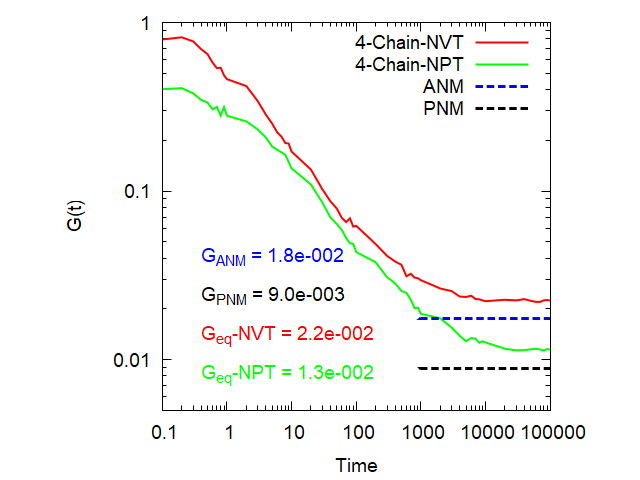
\includegraphics[width=\textwidth]{gt_4chain_comp.png}
					% \includegraphics<2>[width=\textwidth]{gt_NPT_mod.png}
				\end{block}
		\end{columns}
		\note{
		\begin{itemize}
			\item 比較のために、NPT条件を利用して、絡み合いの少ない初期状態を作成しました。
			\item calculated $<Z>_{Z1}$ = 0.36
		\end{itemize}
	}
\end{frame}

\begin{frame}
	\frametitle{
		Entanglement effect in Slip-tube Model
	}
	\vspace{-1mm}
	\begin{alertblock}{Entanglement in Slip-tube Model}
		% \begin{columns}[onlytextwidth]
		% 	\column{.8\linewidth}
			\footnotesize
			Theoretical model by Rubinstein\footnote{
				\scriptsize{M. Rubinstein, S. Panyukov, Macromolecules, 35, 6670 (2002)}
				}
			\vspace{-3mm}
			\scriptsize
			\begin{align*}
				G_c = \nu k_B T \left(1-\dfrac{2}{\phi} \right), \quad G_e = \dfrac{4}{7} \nu k_B T L \\
				% &\text{where $\nu$ is the number density of network chains,} \\
				\text{and L is the number of slip-links per network chain}
			\end{align*}
	\end{alertblock}
	\vspace{2mm}
	\centering
			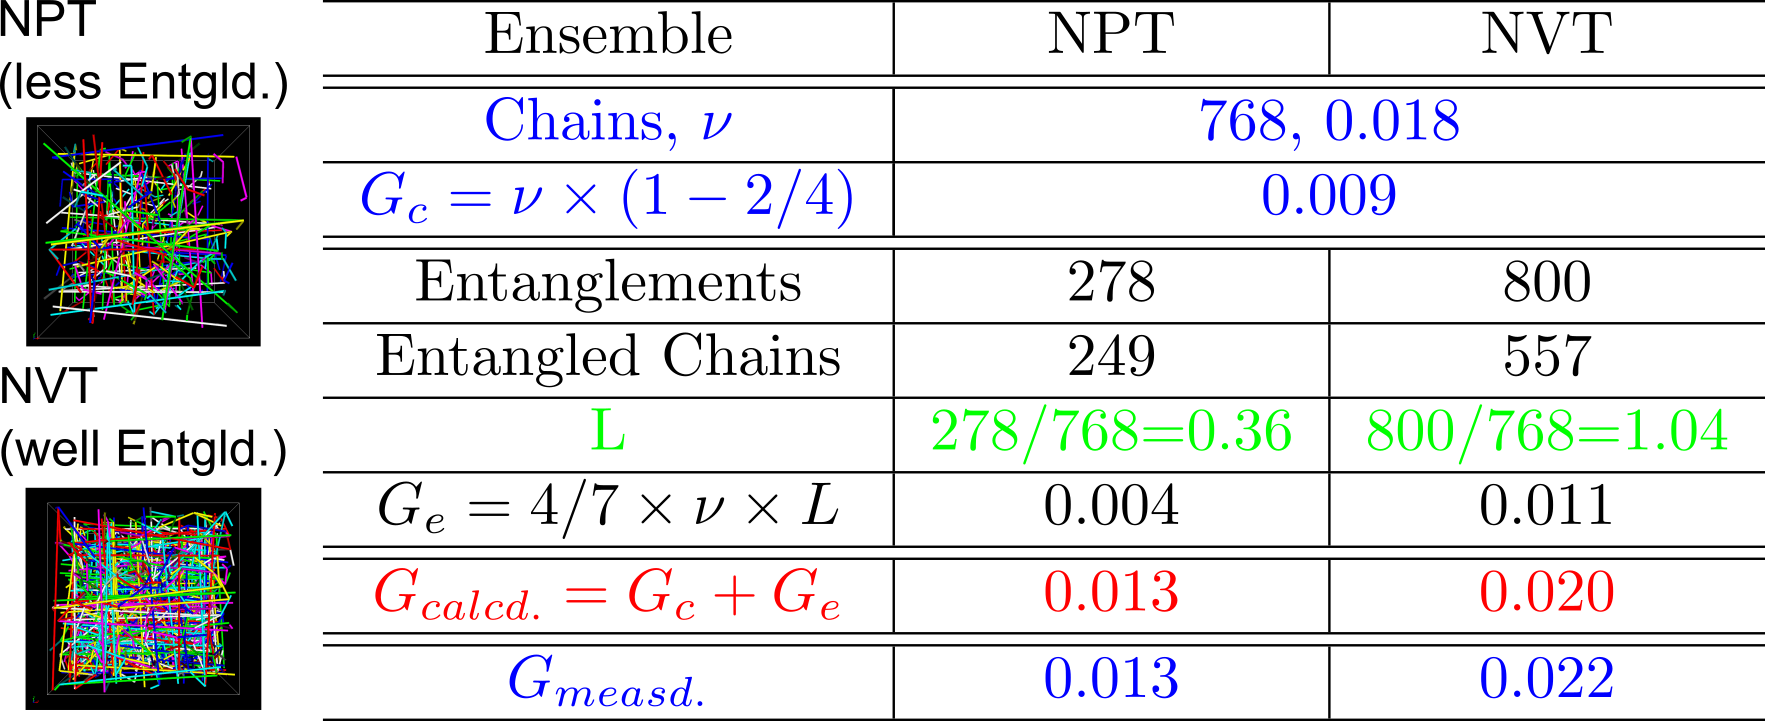
\includegraphics[width=.9\textwidth]{Entanglement_Comp.png}
	\scriptsize
	\note{
		\begin{itemize}
			\item Slip-tube model による見積もりとこれら二つとの比較はよい一致を示しました。
			\item \textcolor{red}{(POINT left two)}
		\end{itemize}
	}
\end{frame}

\subsection{Relaxation in KG Networks}
\begin{frame}
	\frametitle{
		G(t) for Step Shear and Dynamic Rheo-Spectrum
	}
	\vspace{-2mm}
	\begin{columns}[c, onlytextwidth]
		\column{.48\linewidth}
			\begin{block}{G(t) for Step Stretch}
				\centering
					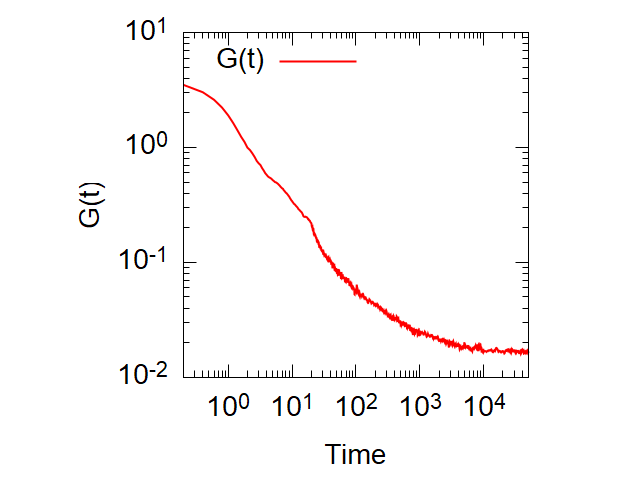
\includegraphics[width=\textwidth]{gt_4chain_N50_stepstretch.png}
			\end{block}
		\column{.48\linewidth}
			\begin{exampleblock}{Dynamic Viscoelastics}
				\centering
					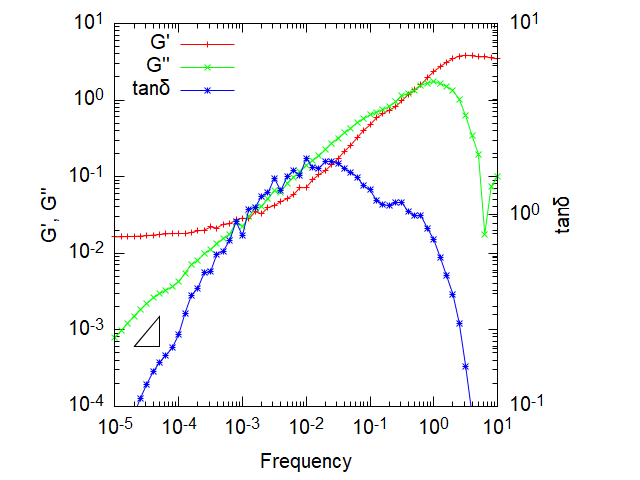
\includegraphics[width=\textwidth]{gw_4chain_N50_stepstretch.png}
			\end{exampleblock}
	\end{columns}

	\begin{block}{Conditions}
		\begin{itemize}
			\item 4-Chain KG-NW(N=50)
			\item Step Stretch: $\lambda = 2$
			\item G(t) is transformed to Dynamic Viscoelastic Spectrum 
		\end{itemize}
	\end{block}

	\note{
		\begin{itemize}
			\item この緩和
			\item G(t) and $\tan \delta$ decayed on a time scale of this region
			\item \textcolor{red}{(POINT)}
			\item it was longer than the longest relaxation time of homo-polymers of comparable length.
			\item This prolonged relaxation time can be attributed to the reduced mobility of the cross-linking points due to the network structure
		\end{itemize}
	}
\end{frame}

\begin{frame}
	\frametitle{Mechanical Hysteresis Loss}
	\vspace{-2mm}
	\begin{columns}[c, onlytextwidth]
		\column{.48\linewidth}
			\begin{exampleblock}{Dynamic Viscoelastics}
				\centering
					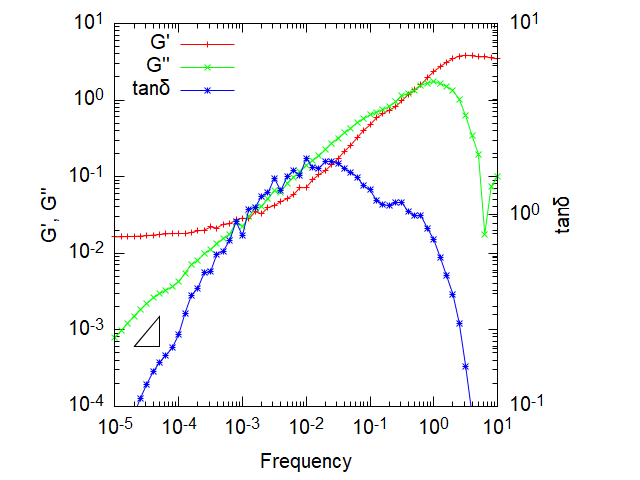
\includegraphics[width=\textwidth]{gw_4chain_N50_stepstretch.png}
			\end{exampleblock}
			\column{.48\linewidth}
			\begin{alertblock}{Hysteresis by Cyclic Shear}
				\centering
					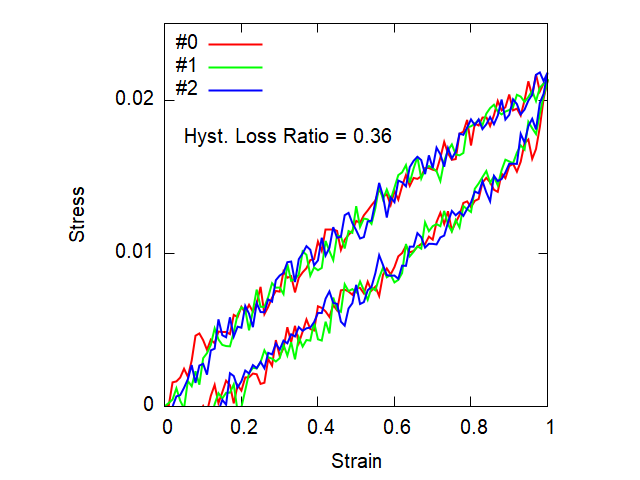
\includegraphics[width=\textwidth]{CyclicDeform_4chain_N50_rate5e-5.png}
			\end{alertblock}
	\end{columns}

	\begin{block}{Conditions}
		\begin{itemize}
			\item 4-Chain KG-NW(N=50)
			\item Cyclic Shear: $\gamma = 1$, $\dot{\gamma} = 5e^{-5}$
		\end{itemize}
	\end{block}

	\note{
		\begin{itemize}
			\item Around this region
			\item \textcolor{red}{(POINT)} 10-5
			\item Hysteresis loss was checked using deformation rate of $\dot{\gamma} = 5e^{-5}$
			\item rather high hysteresis loss was found 0.36
			\item this result should concern with the longer relaxation time 
			\item Network connectivity should affect the nature of hysteresis loss.
		\end{itemize}
	}
\end{frame}


% \begin{frame}
% 	\frametitle{4-Cain NW のせん断変形時のヒステリシス}
% 	\begin{itemize}
% 		% \item 変形速度の低減により、$\gamma<1$ 程度の小さなひずみでは Phantom Network Model:PNM に漸近
% 		\item PNM へと漸近する変形速度 ($\dot{\gamma} = 2e^{-4}$) で複数回の連続した変形に対しても迅速な回復を伴った力学的ヒステリシス (Hysteresis loss $\simeq$ 0.34) を示した。
% 	\end{itemize}

% 	\begin{columns}[totalwidth=\linewidth]
% 		\column{.5\textwidth}
% 			\centering
% 				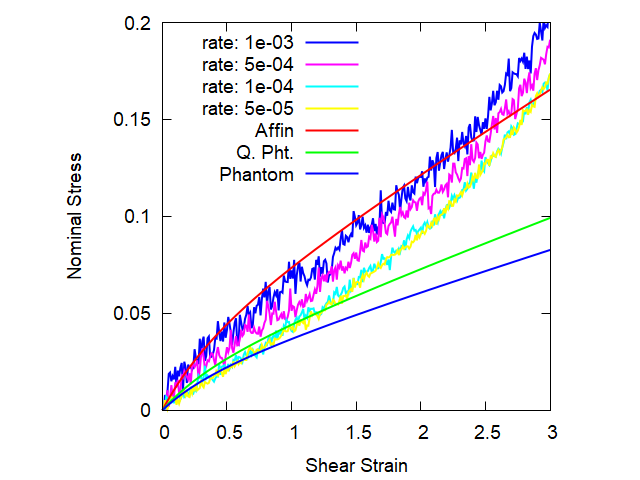
\includegraphics[width=\textwidth]{Shear_Random_4chain_N20.png}
% 				Stress-Strain Curves for 4-chain NW 
% 		\column{.5\textwidth}
% 			\centering
% 				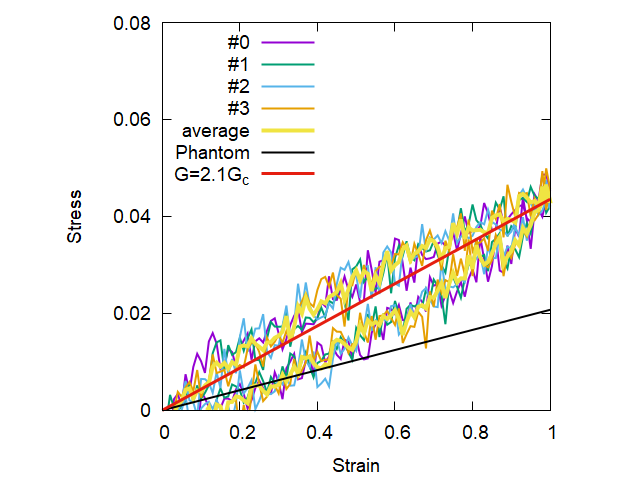
\includegraphics[width=\textwidth]{CyclicDeform_4chain_rate_2e-4.png}
% 				Hysteresis Response with Cyclic Deformations
% 		\end{columns}
% \end{frame}


% \begin{frame}
% 	\frametitle{各種の変形条件での力学的ヒステリシス}
% 		\centering
% 			\includegraphics[width=\textwidth]{hyst_shear_all.png}
% 			Hysteresis losses for valid shear rate and maximum deformation
% \end{frame}

% \begin{frame}
% 	\frametitle{ヒステリシスロス}
% 	\begin{itemize}
% 		\item 変形速度の低下に伴いヒステリシスロスは減少
% 		\item \textcolor{red}{$\dot{\gamma} \sim 1e^{-5}$ 程度のオーダーの時間スケールで消失}
% 	\end{itemize}
% 			\centering
% 				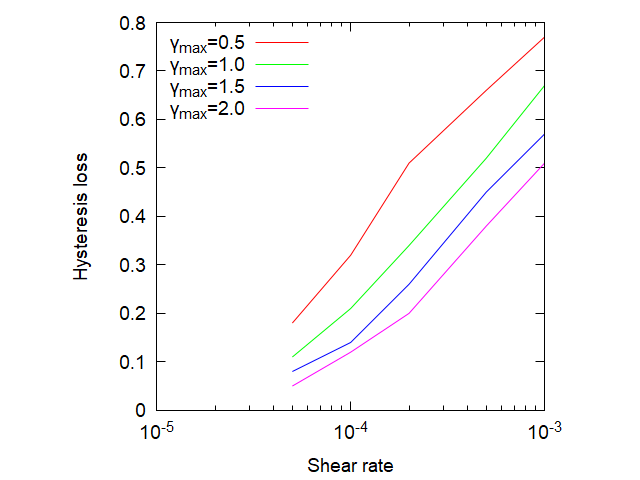
\includegraphics[width=.6\textwidth]{hyst_shear.png}\\
% 					Comparison of Hysteresis losses for 4-Chain NW
% \end{frame}

\begin{frame}
	\frametitle{ストランドの最長緩和時間}
	\begin{exampleblock}{最長緩和時間 ($\tau$) を評価}
		\begin{columns}[totalwidth=\linewidth]
			\column{.65\textwidth}
			\begin{itemize}
				\item ストランドのラウスモード(p=1)の自己相関関数 $C_p(t)$
				\small
				\begin{align*}
					C_p(t) = \langle X_p(t)X_p(0) \rangle/\langle X_p^2 \rangle
				\end{align*}
				\normalsize
				\item 相関関数の振る舞い
				\begin{itemize}
					\item 長時間極限で一定値に収束
					\item 空間的な拘束のため
					\item $C_p(\infty)$ を差し引いて評価
					\small
					\begin{align*}
						\textcolor{red}{\tau \simeq 6.5e^{4}}
					\end{align*}
					\normalsize
				\end{itemize}
			\end{itemize}
			\column{.33\textwidth}
				\centering
					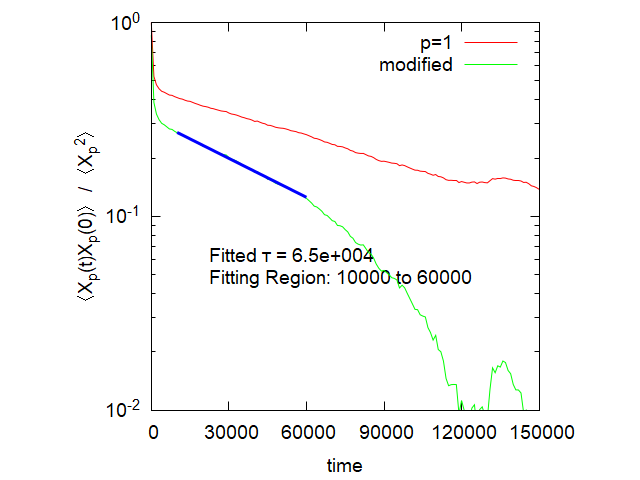
\includegraphics[width=\textwidth]{Xp_1_org.png}\\
					\scriptsize{$C_{p1}(t)$ for equilibrated structure}
		\end{columns}
	\vspace*{2mm}
		\alert{ヒステリシスロスが消失する変形速度 ($\sim 1e^{-5}$) と対応}
	\end{exampleblock}
		
\end{frame}

\begin{frame}
	\frametitle{Effect of Strand Length for Shorter KG Chain}
	\begin{itemize}
		\item For Phantom Chain
		\begin{itemize}
			\item Longer Strand resulted in lower Modulus
		\end{itemize}
		
		\item KG Chain 
		\begin{itemize}
			\item Proper Length was found for Low Modulus
			\item which implies proper restriction for JP
		\end{itemize}
		
	\end{itemize}
	% \begin{exampleblock}{最長緩和時間 ($\tau$) を評価}
		\begin{columns}[totalwidth=\linewidth]
			\column{.48\textwidth}
			\centering
					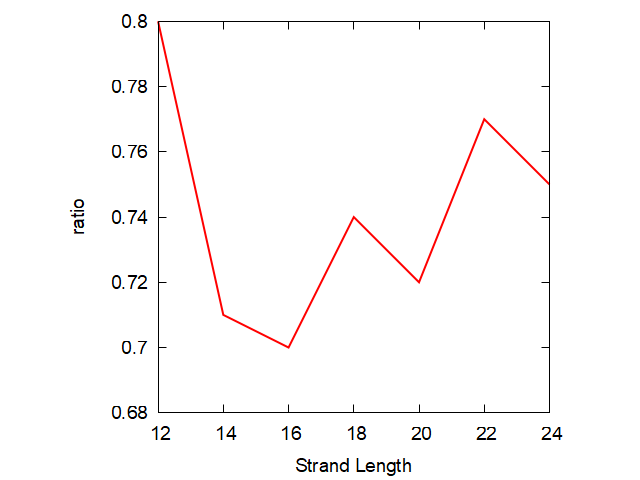
\includegraphics[width=\textwidth]{n_mod.png}\\
					\scriptsize{Strand Length vs. Modulei ratio}
			\column{.48\textwidth}
				\centering
					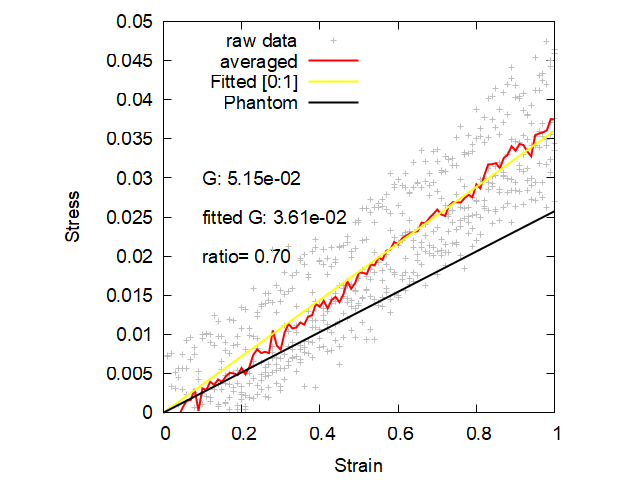
\includegraphics[width=\textwidth]{shear_n16.png}\\
					\scriptsize{Shear Stress for N=16}
		\end{columns}
	% \vspace*{2mm}
	% 	\alert{ヒステリシスロスが消失する変形速度 ($\sim 1e^{-5}$) と対応}
	% \end{exampleblock}
		
\end{frame}


\begin{frame}
	\frametitle{Conclutions}

	\begin{itemize}
		\item Introducing random connectivity, MD simulation studies were carried out.
		\item To investigate the criteria for Phantom Network Model, Two model chains are used.
		\begin{itemize}
			\item Employing phantom chain, basics for PNM is examined.
			\begin{itemize}
				\item Proper strand length is the key for PNM.
				\item Functionality effect was confirmed.
			\end{itemize}
			\item Changing the chain to KG Chain, constraints effects are investigated.
			\begin{itemize}
				\item Trapped Entanglement was explained by Slip-tube Model
				\item Hysteresis 
			\end{itemize}
		\end{itemize}
	\end{itemize}

	\note{
		\begin{itemize}
			\item Introducing random connectivity, MD simulation studies were carried out.
			\item To investigate the criteria for Phantom Network Model, Two model chains are used.
			\begin{itemize}
				\item Employing phantom chain, basics for PNM is examined.
				\begin{itemize}
					\item Proper strand length is the key for PNM.
					\item Functionality effect was confirmed.
				\end{itemize}
				\item Changing the chain to KG Chain, constraints effects are investigated.
				\begin{itemize}
					\item Trapped Entanglement was explained by Slip-tube Model
					\item Hysteresis 
				\end{itemize}
			\end{itemize}
		\end{itemize}
	}

\end{frame}
% \section{ランダムネットワークのせん断変形}
% \subsection{分岐数の異なるネットワークのせん断変形}
% \begin{frame}
% 	\frametitle{シミュレーションによる評価}
% 	\begin{enumerate}
% 		\item KG 鎖 (N=20) 初期構造の確認
% 			\begin{itemize}
% 				\item Kr\"{o}ger らの方法により Z\_1 Code で絡み合いを評価\footnote[1]{
% 					\scriptsize{S. Shanbhag, M. Kr\"{o}ger, Macromol. 40 2897 (2007)}
% 				}
% 				\begin{itemize}
% 					\item 対応するホモポリマーメルトと同程度 ($\langle Z \rangle_{Z1} \simeq 0.15$)
% 					\item 鎖長が短いので絡み合いは少ない
% 				\end{itemize}
% 			\end{itemize}
% 		\item 各種アンサンブル平均を評価
% 			\begin{itemize}
% 				\item ストランド長の分布関数
% 				\item 鎖に沿ったセグメント間距離
% 			\end{itemize}
% 		\item 力学特性の評価
% 			\begin{itemize}
% 				\item 一軸伸張において、生じる応力を評価
% 				\item ステップ変形による応力緩和
% 				\item \alert{Lees-Edwards 条件によりずりせん断}を付与し、\\生じる応力を評価
% 				\item 連続した変形を付与して、ヒステリシスを評価
% 			\end{itemize}	
% 	\end{enumerate}
% \end{frame}

% \begin{frame}
% 	\frametitle{分岐数の異なるネットワークのせん断変形}
% 	\begin{alertblock}{「素抜け鎖」でのランダムネットワーク}
% 		\begin{itemize}
% 			% \item ストランド:す抜け鎖
% 			\item \alert{「排除体積効果および絡み合いのない」}ネットワーク
% 		\end{itemize}
% 	\end{alertblock}
% 	\begin{itemize}
%         \item 分岐数が異なるネットワークのせん断変形力学応答
% 		\item 分岐数によらずPhantom Network Model:PNM へと漸近
% 	\end{itemize}

% 	\begin{columns}[T, onlytextwidth]
% 		\column{.25\linewidth}
% 			\centering
% 			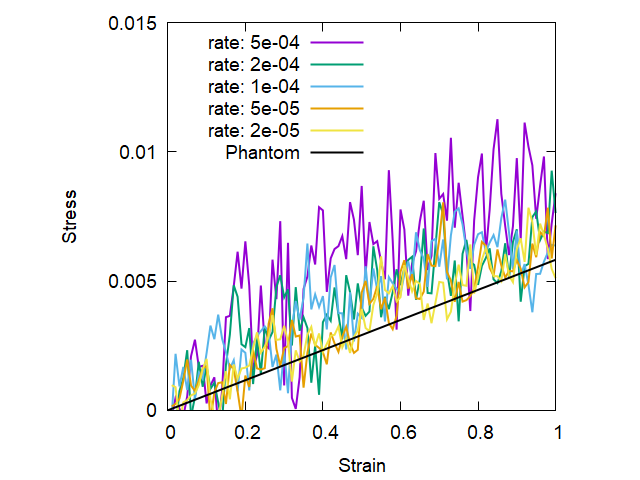
\includegraphics[width=\textwidth]{Shear_Random_3chain_N48.png}
% 			3-Chain NW (N=48)
% 		\column{.25\linewidth}
% 			\centering
% 			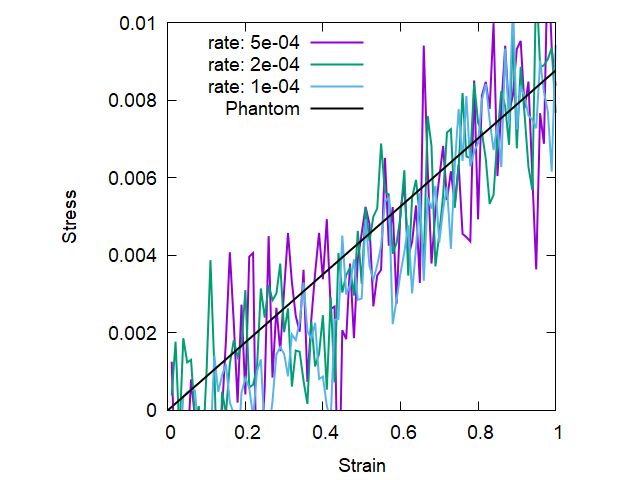
\includegraphics[width=\textwidth]{Shear_Random_4chain_N48.png}
% 			4-Chain NW (N=48)
		
% 		\column{.25\linewidth}
% 		\centering
% 		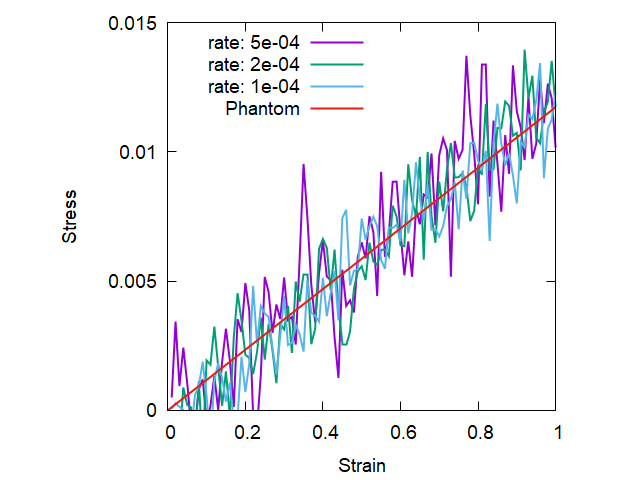
\includegraphics[width=\textwidth]{Shear_Random_6chain_N48.png}
% 		6-Chain NW (N=48)
% 		\column{.25\linewidth}
% 		\centering
% 			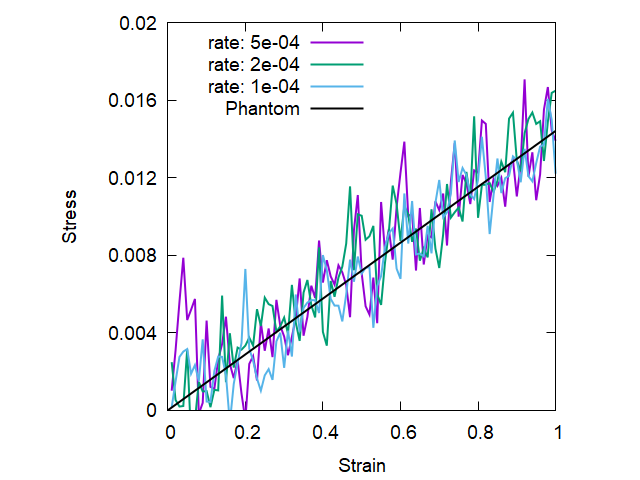
\includegraphics[width=\textwidth]{Shear_Random_5chain_N35.png}
% 			5-Chain NW (N=35)
% 	\end{columns}
% \end{frame}

% \subsection{4-Cain NW のせん断変形時のヒステリシス}
% \begin{frame}
% 	\frametitle{4-Cain NW (KG Chain: N=20) のせん断変形}
% 	\begin{itemize}
% 		% \item 変形速度の低減により、$\gamma<1$ 程度の小さなひずみでは Phantom Network Model:PNM に漸近
% 		\item PNM へと漸近する変形速度 ($\dot{\gamma} = 2e^{-4}$) で複数回の連続した変形に対しても迅速な回復を伴った力学的ヒステリシス (Hysteresis loss $\simeq$ 0.34) を示した。
% 	\end{itemize}

% 	\begin{columns}[totalwidth=\linewidth]
% 		\column{.5\textwidth}
% 			\centering
% 				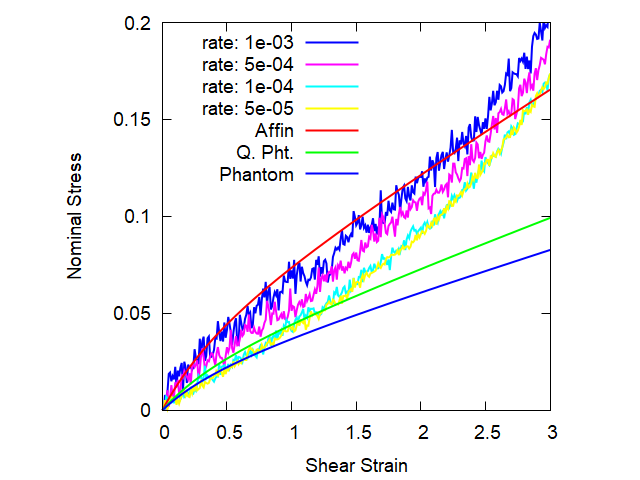
\includegraphics[width=\textwidth]{Shear_Random_4chain_N20.png}
% 				Stress-Strain Curves for 4-chain NW (N=20)
% 		\column{.5\textwidth}
% 			\centering
% 				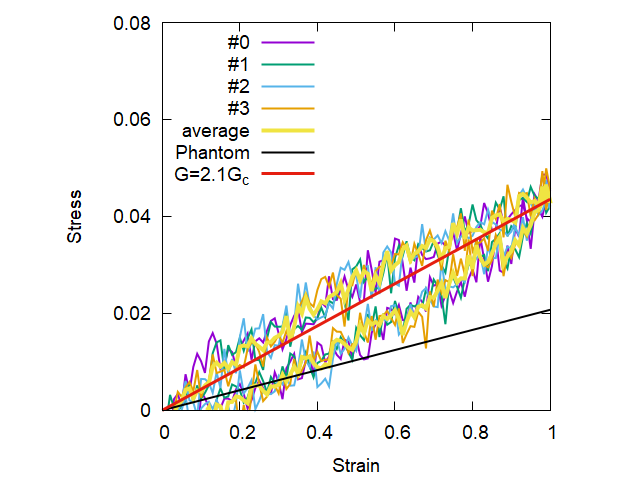
\includegraphics[width=\textwidth]{CyclicDeform_4chain_rate_2e-4.png}
% 				Hysteresis Response with Cyclic Deformations
% 		\end{columns}
% \end{frame}


% \begin{frame}
% 	\frametitle{各種の変形条件での力学的ヒステリシス}
% 		\centering
% 			\includegraphics[width=\textwidth]{hyst_shear_all.png}
% 			Hysteresis losses for valid shear rate and maximum deformation
% \end{frame}

% \begin{frame}
% 	\frametitle{ヒステリシスロス}
% 	\begin{itemize}
% 		\item 変形速度の低下に伴いヒステリシスロスは減少
% 		\item \textcolor{red}{$\dot{\gamma} \sim 1e^{-5}$ 程度のオーダーの時間スケールで消失}
% 	\end{itemize}
% 			\centering
% 				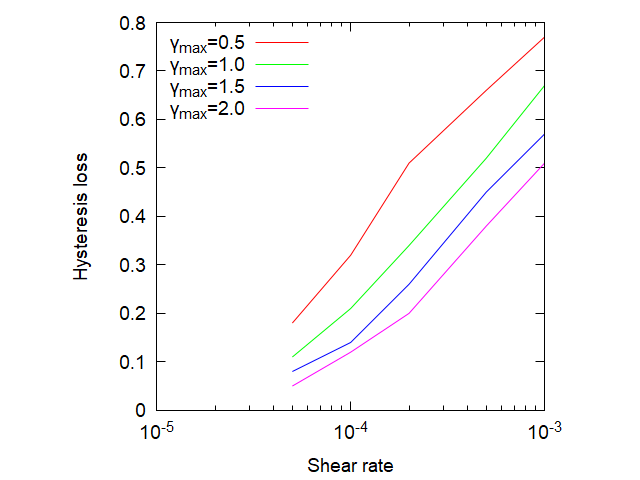
\includegraphics[width=.6\textwidth]{hyst_shear.png}\\
% 					Comparison of Hysteresis losses \\for 4-Chain NW (N=20)
% \end{frame}

% \begin{frame}
% 	\frametitle{ストランドの最長緩和時間}
% 	\begin{exampleblock}{最長緩和時間 ($\tau$) を評価}
% 		\begin{columns}[totalwidth=\linewidth]
% 			\column{.65\textwidth}
% 			\begin{itemize}
% 				\item ストランドのラウスモード(p=1)の自己相関関数 $C_p(t)$
% 				\small
% 				\begin{align*}
% 					C_p(t) = \langle X_p(t)X_p(0) \rangle/\langle X_p^2 \rangle
% 				\end{align*}
% 				\normalsize
% 				\item 相関関数の振る舞い
% 				\begin{itemize}
% 					\item 長時間極限で一定値に収束
% 					\item 空間的な拘束のため
% 					\item $C_p(\infty)$ を差し引いて評価
% 					\small
% 					\begin{align*}
% 						\textcolor{red}{\tau \simeq 6.5e^{4}}
% 					\end{align*}
% 					\normalsize
% 				\end{itemize}
% 			\end{itemize}
% 			\column{.33\textwidth}
% 				\centering
% 					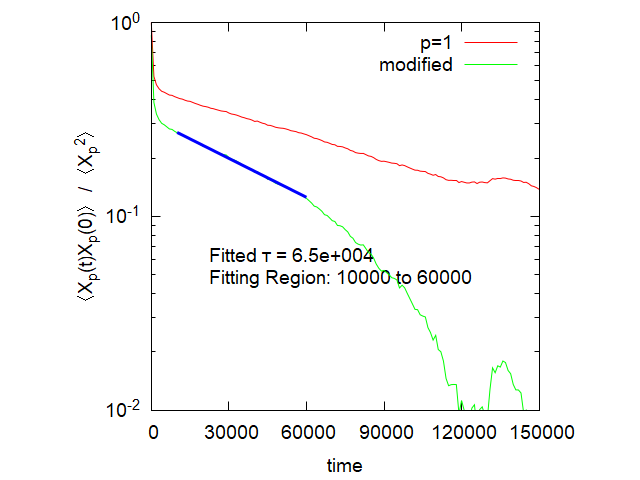
\includegraphics[width=\textwidth]{Xp_1_org.png}\\
% 					\scriptsize{$C_{p1}(t)$ for equilibrated structure}
% 		\end{columns}
% 	\vspace*{2mm}
% 		\alert{ヒステリシスロスが消失する変形速度 ($\sim 1e^{-5}$) と対応}
% 	\end{exampleblock}
		
% \end{frame}

% \subsection{おわりに}
% \begin{frame}
% 	\frametitle{おわりに}
% 		\begin{block}{本発表の内容}
% 			\begin{itemize}
% 				\item ストランド長が揃った分岐数の異なるランダム-\\ネットワーク
% 				\begin{itemize}
% 					\item ずりせん断での力学応答を評価
% 					\item 分岐数に応じたファントムネットワーク挙動を確認
% 				\end{itemize}
% 				\item 迅速な回復を伴った力学的ヒステリシスを確認
% 				\begin{itemize}
% 					\item ストランドの最長緩和時間が長時間化($\tau \simeq 6.5e^{4}$)
% 					\item ヒステリシスロスが消失する変形速度と対応
% 				\end{itemize}
%                \item 今後の検討
%                \begin{itemize}
% 				\item ストランド長および分岐数を変更したものを\\網羅的に検討
% 				\item 今回の知見に基づき、一軸伸張での検討を整理
% 			   \end{itemize}  
% 			\end{itemize}
% 		\end{block}
% \end{frame}

% \setcounter{section}{0}
% %%%%%%%%%%%%%%%%%%%%%%%%%%%%%%%%%%%%%%%%%%%%%%%
% \appendix

% \backupbegin

% \begin{frame}
% 	\LARGE{補足資料}
% \end{frame}
% %%%%%%%%%%%%%%%

% \section{背景}

% \subsection{背景}

% \begin{frame}
% 	\frametitle{高分子材料への期待と不安}
% 	地球温暖化対策の CO$_2$ 削減へ向けて、\\
% 	「自動車を中心とした運送機器の抜本的な軽量化」が提唱
% 	\begin{block}{高分子材料への期待}
% 		\begin{itemize}
% 			\item 鉄鋼主体$ \Rightarrow$ \textcolor{green}{高分子材料を含むマルチマテリアル化}
% 			\item 高分子材料によるマルチマテリアル化のポイント
% 				\begin{itemize}
% 					\item \alert{高い比強度}の有効利用
% 					\item 特徴を生かした適材適所 $\Leftrightarrow$ 適切な接合方法の選択
% 						\begin{itemize}
% 							\item {\color{red} 「接着接合」}への高分子の利用
% 							\item {\color{red} 「柔らかさを生かした弾性接着接合」}
% 						\end{itemize}
% 				\end{itemize}
% 		\end{itemize}
% 	\end{block}
% 	\begin{alertblock}{柔軟材料としてゴム材料に注目}
% 		\begin{itemize}
% 			\item しなやかな強さを有する材料
% 			\item {\color{blue}強度や耐久性の定義が不明確(特に疲労破壊に対して)}
% 		\end{itemize}
% 	\end{alertblock}
% \end{frame}

% \subsection{ゴムの破壊について}

% \begin{frame}
% 	\frametitle{ガラス状態の高分子材料の疲労と破壊}
% 		\begin{columns}[totalwidth=1\textwidth]
% 			\column{.52\textwidth}
% 				\begin{block}{破壊のモード(巨視的)}
% 					脆性破壊 $\Leftrightarrow$ 延性破壊\\
% 					脆性破壊は、降伏前にミクロな\\クラックが進展した破壊
% 				\end{block}
% 			\column{.42\textwidth}
% 				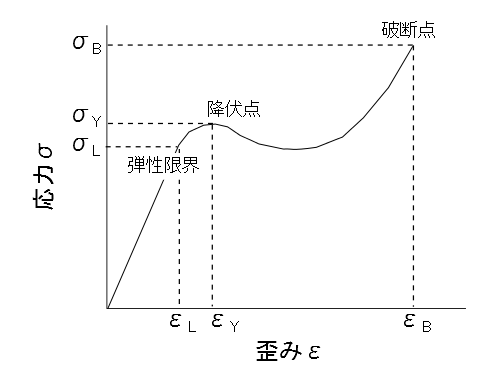
\includegraphics[width=.8\textwidth]{S_S_Curve.png}
% 		\end{columns}
% 		\begin{exampleblock}{降伏と劣化}
% 			\begin{itemize}
% 				\item 靭性向上のため
% 				\begin{itemize}
% 					\item {\color{red} 局所的な降伏}が必須。\\(クレイズのような局所的な破壊も)
% 					\item 一般に、高分子材料の{\color{red} 降伏は不可逆}。
% 				\end{itemize}
% 				\item 降伏による劣化
% 					\begin{itemize}
% 						\item 降伏 $\Leftrightarrow$ {\color{red} 本質的には、少しずつ破壊。}
% 						\item {\color{red} 破壊領域への水分の浸透 $\Leftarrow$ 長期耐久性の欠如}
% 					\end{itemize}
% 			\end{itemize}
% 		\end{exampleblock}
% \end{frame}

% \begin{frame}
%     \frametitle{破壊工学の考え方}
% 	\vspace{-2mm}
%     \begin{exampleblock}{破壊工学の考え方}
% 		\begin{itemize}
% 			\item 系中に\alert{クラックが存在することを前提}
% 			\begin{itemize}
% 				\item グリフィスの条件(脆性材料)\footnote[1]{
% 					A. A. Griffith, Phil. Trans. Roy. Soc. London, A221, 163 (1921)
% 					}
% 					\item 弾塑性材料の延性破壊への拡張\footnote[2]{
% 						G.R.Irwin, J. Appl. Mech., 24, 361 (1957)
% 						}
% 			\end{itemize}
% 		\end{itemize}
% 	\end{exampleblock}
% 	\vspace{-2mm}
% 	\begin{columns}
% 		\column{.58\textwidth}
% 			\begin{itemize}
% 				\item
% 				応力拡大係数 $K_I$ で評価
% 				\footnotesize
% 				\begin{align*}
% 				K_{I} = \sigma \sqrt{\pi c}
% 				\end{align*}
% 				\normalsize
% 				\item 
% 				先端での局所降伏領域: d\\
% 				$\Rightarrow$ 降伏応力 $\sigma_Y$ に反比例
% 				\footnotesize
% 				\begin{align*}
% 				d \propto \left( \dfrac{K_I}{\sigma_Y} \right)^2
% 				\end{align*}
% 				\normalsize
% 			\end{itemize}
% 		\column{.4\textwidth}
% 			\centering
% 			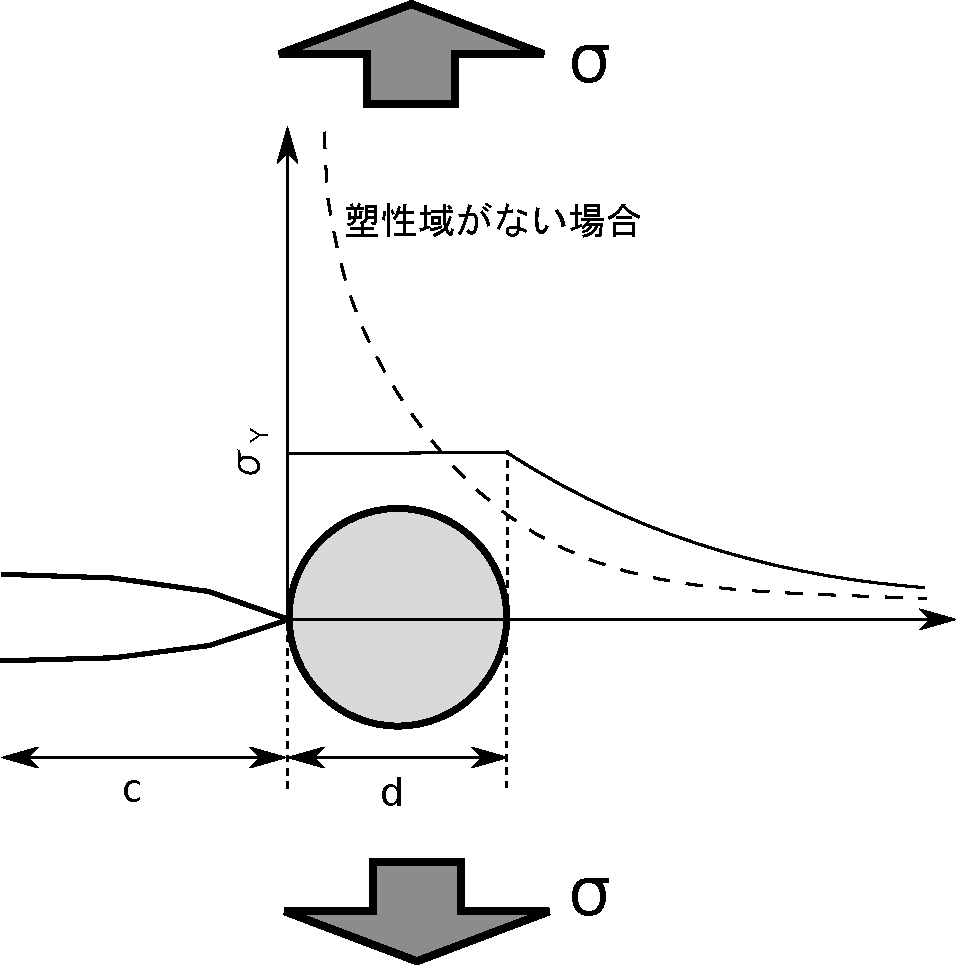
\includegraphics[width=.82\textwidth]{./Crack_Yield.pdf}
% 		\end{columns}
% \end{frame}

% \begin{frame}
% 	\frametitle{ゴムの破壊と時間温度換算則}
% 		\begin{alertblock}{ゴムの破壊について}
% 			クラック先端での大変形を伴う非線形現象だが、\\時間温度換算則の成立が多数報告\footnote{
% 				Smith T., Stedry P., J. Appl. Phys., 31 1892 (1960)
% 			}
% 		\end{alertblock}
% 		\vspace{-2mm}
% 		\begin{columns}[T, totalwidth=\textwidth]
% 			\column{.48\textwidth}
% 				亀裂先端近傍での大変形
% 				\vspace{-3mm}
% 				\begin{center}
% 					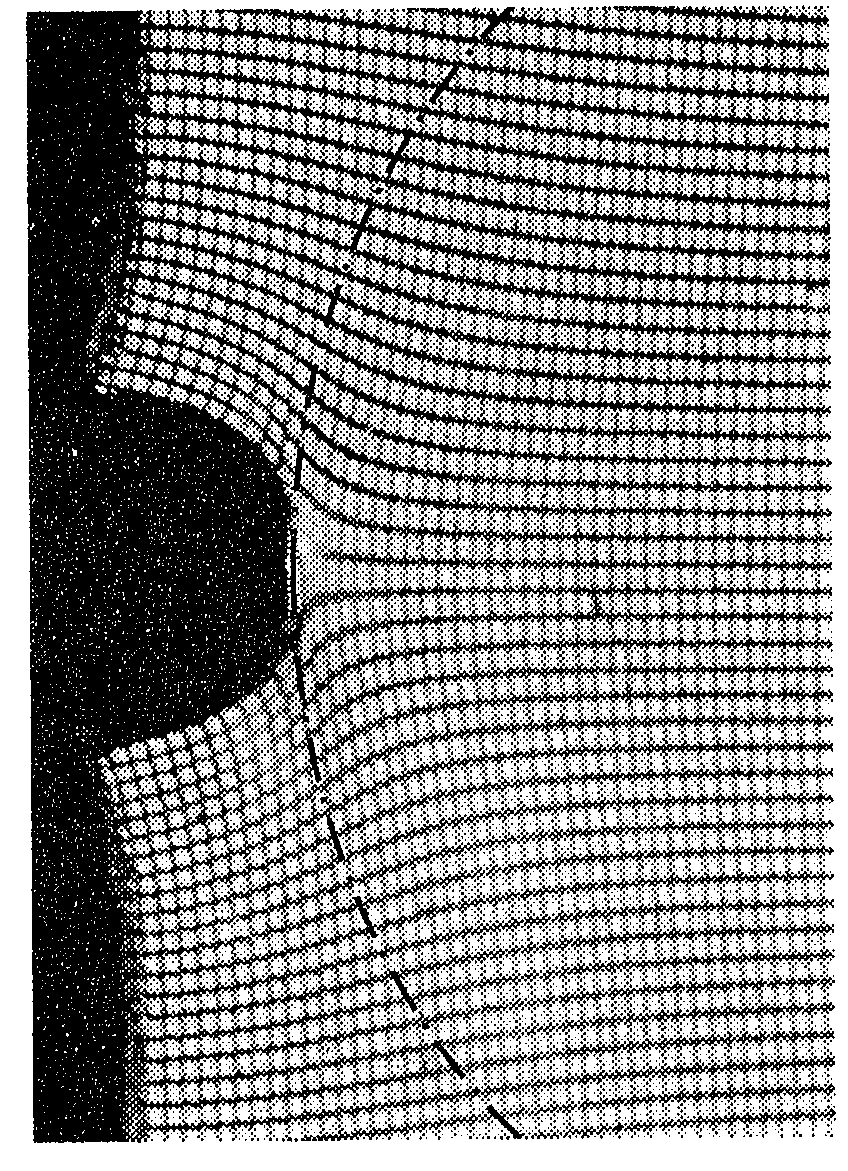
\includegraphics[width=.55\textwidth]{rubber_crack.png}
% 				\end{center}
% 			\column{.48\textwidth}
% 				時間温度換算則の成立
% 				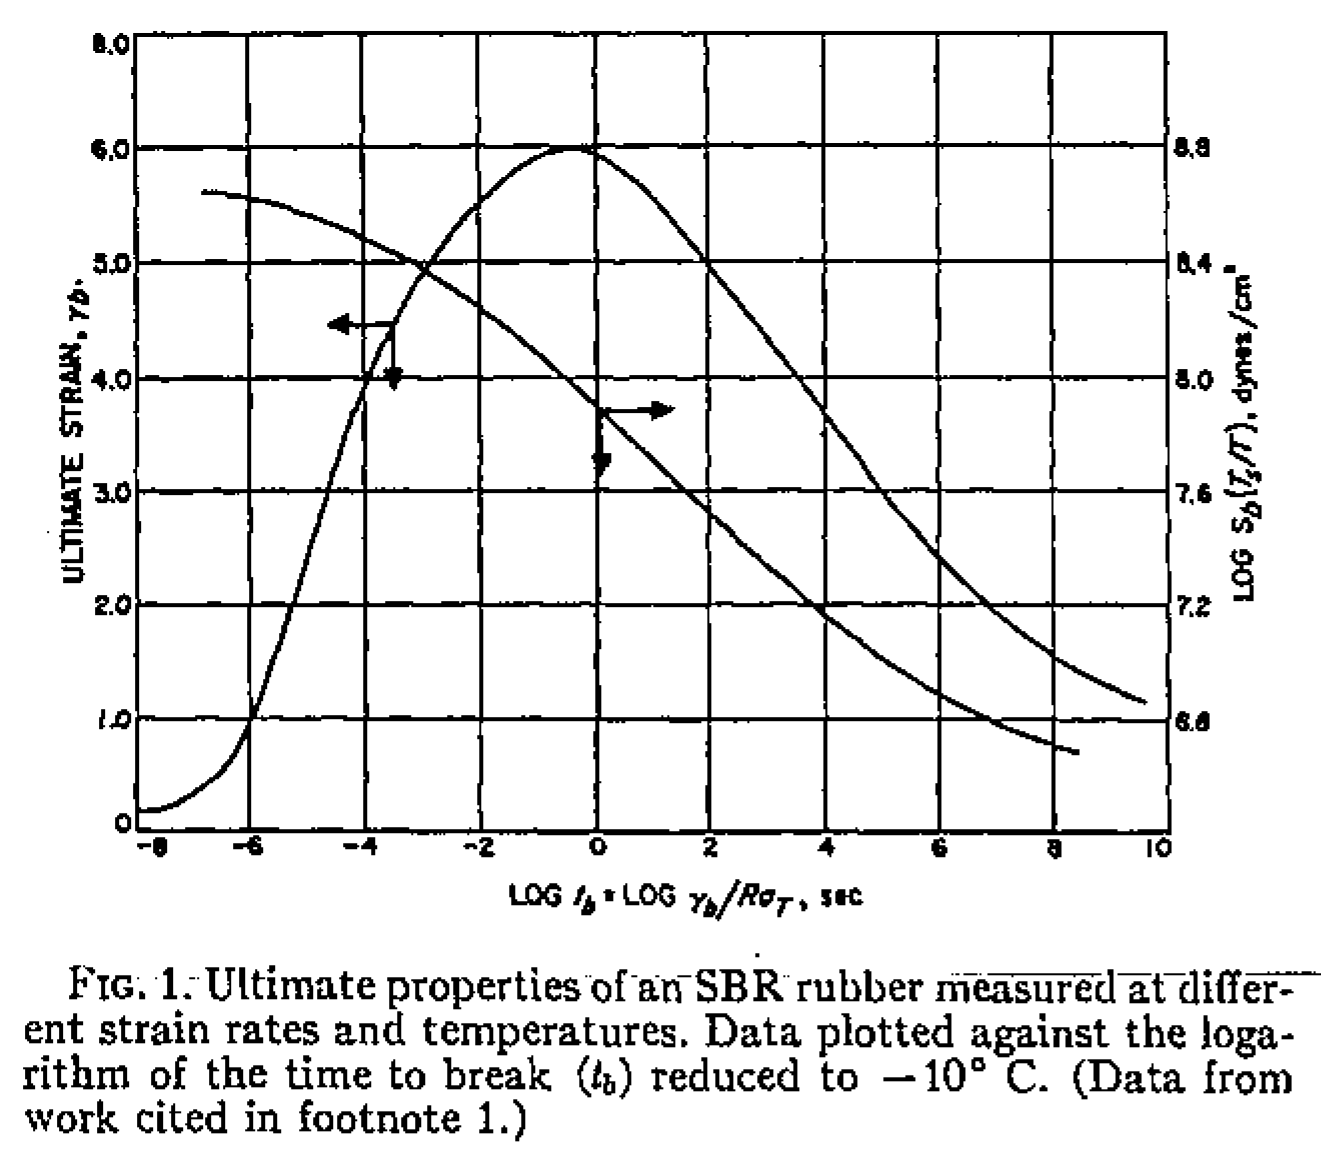
\includegraphics[width=.8\textwidth]{Time_Temp_2.png}
% 		\end{columns}
% \end{frame}

% \begin{frame}
%     \frametitle{ゴムの破断強度の時間温度依存}
% 	\vspace{-2mm}
%     \begin{columns}[T, totalwidth=\textwidth]
%     \column{.53\textwidth}
%     \begin{itemize}
% 		\item \alert{粘弾性極限において\footnote[1]{
% 			G.J. Lake and A.G. Thomas, \\R. Soc. Lond. A300, 108 (1967)
% 		}}\\
% 		(高温・低速)
% 	\end{itemize}
%     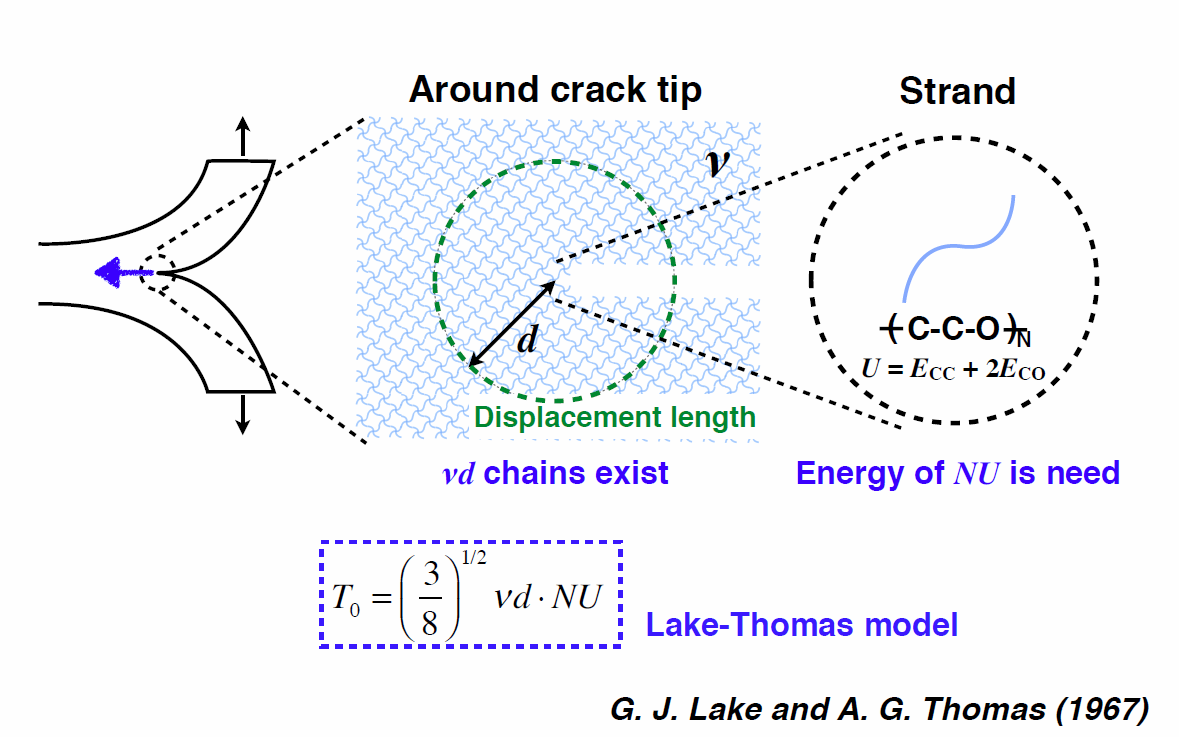
\includegraphics[width=\textwidth]{Lake_Thomas.png}
    
%     \column{.45\textwidth}
%     \begin{itemize}
% 		\item 変形速度、温度に依存\\
% 		\alert{破壊包絡線\footnote[2]{
% 			Smith T., Stedry P., \\J. Appl. Phys. (1960) 31 1892
% 		}}
% 	\end{itemize}
% 	\begin{center}
% 		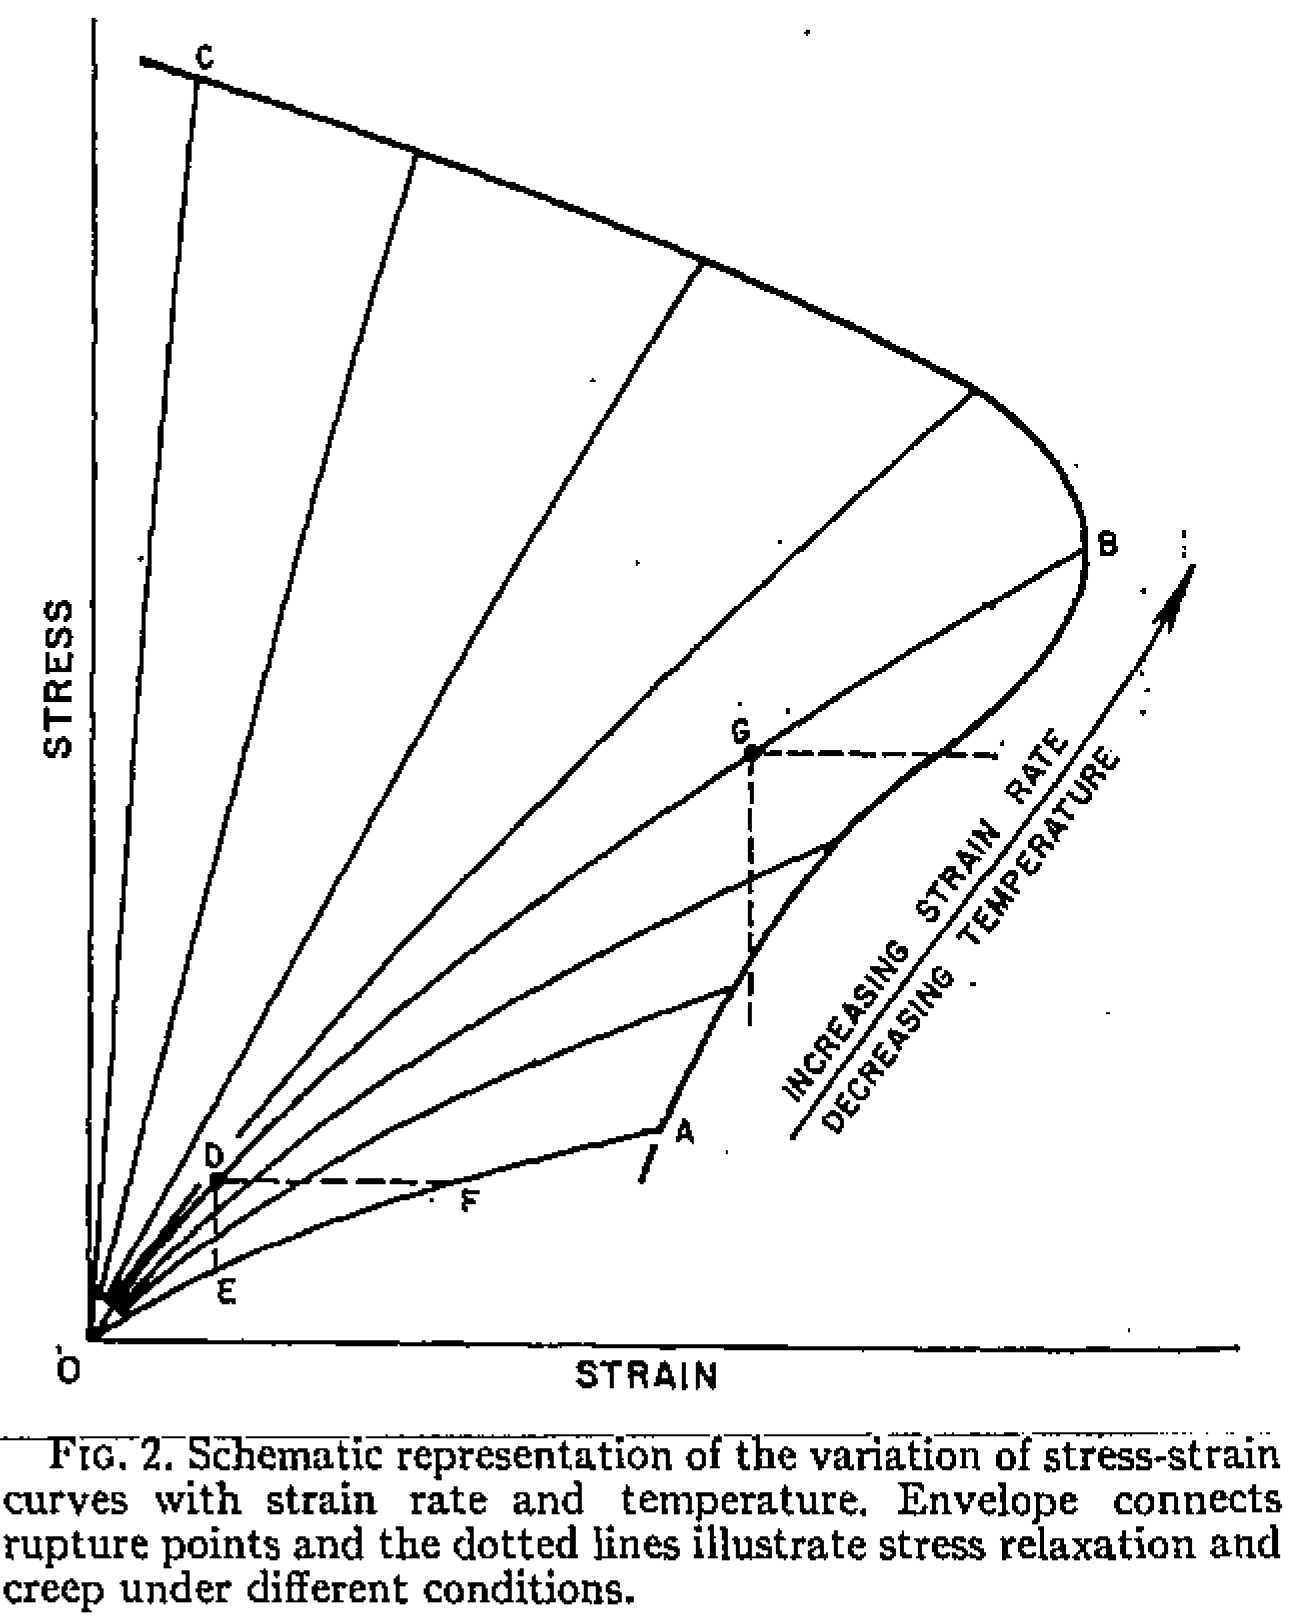
\includegraphics[width=.4\textwidth]{Time_Temp_3.png}
% 	\end{center}
%     \end{columns}
%     \begin{alertblock}{ゴムの引き裂きエネルギー}
% 		\vspace{-2mm}
% 		\begin{align*}
% 			&\mathcal{T}=\mathcal{T}_0 \times {\color{red}\Phi}(\dot{c}, T, \epsilon_0) \\
% 			&\text{where $\dot{c}$ is crack velocity and $\epsilon_0$ is applied strain}
% 		\end{align*}
%     % $\mathcal{T}=\mathcal{T}_0 \Phi(\dot{c}, T, \epsilon_0)$
%     \end{alertblock}
% \end{frame}


% \begin{frame}
% 	\frametitle{Andrews 理論}
% 	\vspace{-2mm}
% 	\begin{exampleblock}{Andrews 理論}
% 		\begin{columns}[totalwidth=1\textwidth]
% 			\column{.68\textwidth}
% 			\begin{itemize}
% 			\item クラック近傍の応力場\footnote{
% 					Andrews, E. H. and Fukahori, Y., \\J. of Mat. Sci., 12, 1307 (1977)
% 					}
% 					\begin{itemize}
% 						\item \textcolor{blue}{Loading 場}と\textcolor{red}{Unloading 場}
% 						\item クラック進展時に遷移
% 					\end{itemize}
% 			\item ヒステリシスロスを有する材料では
% 				\begin{itemize}
% 				\item
% 				\alert{この差}が、全体の変形に要した\\エネルギーの多くを\alert{散逸}
% 				\item
% 			鎖の破断へのエネルギーが低減 \\$\Rightarrow$ \alert{強靭さの起源。}
% 				\end{itemize}	
% 			\item \textcolor{green}{実験的に、$\Phi$ を求めている。}
% 			% \item \alert{ミクロな緩和現象}がマクロな耐久性向上と繋がる?
% 			\end{itemize}
		
% 			\column{.3\textwidth}
% 			\centering
% 			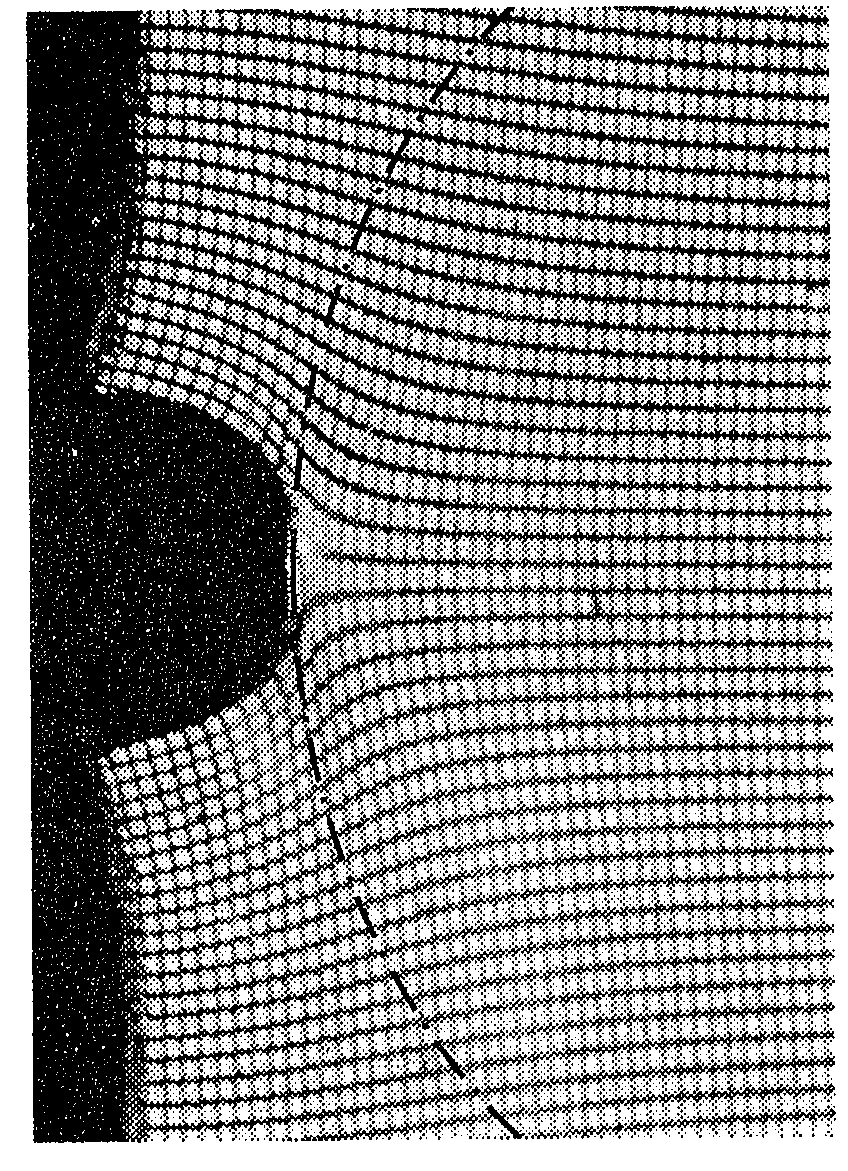
\includegraphics[width=.7\textwidth]{rubber_crack.png}
% 			\vspace{3mm}
% 			\includegraphics[width=.7\textwidth]{./crack.png}
% 		\end{columns}
% 	\end{exampleblock}
% \end{frame}


% \begin{frame}
% 	\frametitle{力学的ヒステリシス}
% 		\vspace{-2mm}
% 		\begin{exampleblock}{力学的ヒステリシス}
% 			\begin{columns}[totalwidth=\textwidth]
% 				\column{.7\textwidth}
% 					\begin{itemize}
% 						\item
% 						\textcolor{red}{Unloading} 時の応力が低下
% 						\item
% 						ヒステリシスロス$\Rightarrow$エネルギー散逸
% 					\end{itemize}
% 				\column{.3\textwidth}
% 					\centering
% 					\includegraphics[width=.6\textwidth]{hysteresis_curve.png}
% 			\end{columns}
% 			\end{exampleblock}
% 			\vspace{-2mm}
% 			\begin{block}{ヒステリシス発生の起源}
% 				\begin{itemize}
% 					\item フィラーの添加効果\footnote{
% 						\scriptsize{K. A. Grosch et al. Rub. Chem. and Tech.41, 1157 (1968)}
% 					}
% 					\item フィラー近傍でのナノキャビティーの開閉\footnote{
% 						\scriptsize{H. Zhang et al. Macromol. 46, 900 (2013)}
% 					}
% 				\end{itemize}
% 			\end{block}
% 			\vspace{-2mm}
% 			\begin{alertblock}{疲労破壊も考慮すると}
% 				\begin{itemize}
% 					\item \alert{可逆的}であることが望ましい。\textcolor{blue}{$\neq$ 犠牲結合}
% 					\item 変形の周期に対応できるように、\alert{回復速度}も重要。
% 				\end{itemize}
% 			\end{alertblock}
% \end{frame}


% %%%%%%%%%%%%%%%%%


% \subsection{ゴムのモデル化}

% \begin{frame}
% 	\frametitle{ひずみ不変量}

% 	主伸張比 $\lambda$ を用いて以下のように、\\ひずみの第1不変量、第2不変量、第3不変量
% 		\begin{align*}
% 			I_1 &= \lambda_1^2 + \lambda_2^2 + \lambda_3^2 \\
% 			I_2 &= \lambda_1^2\lambda_2^2 + \lambda_2^2\lambda_3^2 + \lambda_3^2\lambda_1^2 \\
% 			I_1 &= \lambda_1^2\lambda_2^2\lambda_3^2
% 		\end{align*}

% 	どの座標系においても不変であり、\\物理的には以下のように解釈される。
% 	\begin{description}
% 		\item [ひずみの第1不変量]
% 		長さの変化量
% 		\item [ひずみの第2不変量]
% 		表面積の変化量
% 		\item [ひずみの第3不変量]
% 		体積の変化量
% 	\end{description}
% \end{frame}




% \begin{frame}
% 	\frametitle{架橋点近傍の拘束状態に基づく二つのモデル}
% 	\vspace{-3mm}
% 		\begin{columns}[totalwidth=1\textwidth]
% 			\column{.45\textwidth}
% 				\begin{block}{ストランドと架橋点}
% 					\includegraphics[width=\textwidth]{JP_vicinity.png}
% 					架橋点はストランド経由で直接連結した架橋点以外の、
% 					\alert{近接する多数のストランド(図中の×)に囲まれている。}
% 				\end{block}
% 			\column{.52\textwidth}
% 			\begin{itemize}
% 				\item \textcolor{blue}{``Affine NW Model''}\\[1mm]
% 					架橋点が巨視的変形と相似に移動。(Affine 変形)
% 					\vspace{-3mm}
% 					\footnotesize
% 					\begin{align*}
% 						&G=\nu k_B T \\
% 						&\text{$\nu$ は、ストランドの数密度}
% 					\end{align*}
% 					\normalsize
% 				\item \textcolor{red}{``Phantom NW Model''}\\[1mm]
% 					架橋点が大きく揺らぎ、ずり弾性率($G$)が低下\footnote{
% 						P. J. Flory, Proc. R. Soc. London. Series A, 351, 351 (1976)
% 					}。
% 					\vspace{-3mm}
% 					\footnotesize
% 					\begin{align*}
% 						&G={\color{red}\xi} \nu k_B T \\
% 						&{\color{red}\xi= 1 -\dfrac{2}{f}}\\
% 						&\text{$f$ は架橋点の分岐数}
% 					\end{align*}
% 			\end{itemize}
% 		\end{columns}
% \end{frame}

% % \subsection{ファントムネットワークの理論}
% \begin{frame}
% 	\frametitle{Phantom Network Model (System size effect)}
% 		\begin{columns}[totalwidth=1\textwidth]
% 			\column{.48\textwidth}
% 				\begin{block}{末端の壁面固定の効果}
% 				\begin{itemize}
% 					\item 壁面に末端が固定
% 						\begin{itemize}
% 							\item $n$ 本のストランド
% 							\item セグメント数: $N$
% 							\item 他端が架橋点($\bm{r}$)
% 						\end{itemize}
% 					\item 架橋点の運動性
% 						\begin{itemize}
% 							\item 壁と$N/n$ 個の短い\\ストランドと等価
% 							\item 壁の移動(変形)の影響減少
% 						\end{itemize}
% 				\end{itemize}
% 				% \vspace{-2mm}
% 				\begin{center}
% 					\includegraphics[width=.8\textwidth]{phantom-1.png}
% 				\end{center}
% 				\end{block}
% 			\column{.48\textwidth}
% 				\begin{exampleblock}{内部の鎖が受ける変形}
% 					\begin{itemize}
% 						\item システム内部の鎖の末端はガウス分布
% 						\item 壁面固定の末端からの変形が内部に伝達して、
% 					\end{itemize}
% 					\tiny
% 					\begin{align*}
% 						&G=\xi \nu k_BT \\
% 							&\begin{cases}
% 							\xi_{\infty} = 1-\dfrac{2}{f} \;\; \text{System}\sim \infty \\[8pt]
% 							\xi_{s} = \dfrac{f-1}{f+1} \;\; \text{Small Limit}
% 							\end{cases}
% 					\end{align*}
% 					\vspace{-3mm}
% 					\begin{center}
% 						\includegraphics[width=0.5\textwidth]{phantom.png}
% 					\end{center}
% 				\end{exampleblock}
% 		\end{columns}
% \end{frame}
% %%%%%%%%%%%%%%%%%%%%%%%%%%
% % \subsection{ファントムネットワークの振る舞い}
% \begin{frame}
% 	\frametitle{ファントムネットワークのゆらぎ}
% 		\begin{block}{ゆらぎの入ったポテンシャル}
% 			\begin{itemize}
% 				\item ストランドの末端間ベクトル $\bm{R}_{nm}$ を、\\架橋点の位置ベクトル $\bm{r}_n$ を用いて、
% 					\footnotesize
% 					\begin{equation*}
% 						\bm{R}_{nm} \equiv \bm{r}_n-\bm{r}_m
% 					\end{equation*}
% 					\normalsize
% 				\item 系のポテンシャルエネルギーは、
% 					\footnotesize
% 					\begin{equation*}
% 						U=\dfrac{k}{2} \sum_{\langle nm \rangle} \bm{R}_{nm}^2
% 					\end{equation*}
% 					\normalsize
% 				\item これは、自然長で決まる定数項と、ゆらぎに起因した第二項に分割でき、その和で以下となる。
% 					\footnotesize
% 					\begin{equation*}
% 						U=\dfrac{k}{2} \sum_{\langle nm \rangle} {\bm{R}_{nm}^{(0)}}^2 + \dfrac{k}{2} \sum_{\langle nm \rangle} \Delta \bm{R}_{nm}^2
% 					\end{equation*}
% 					\normalsize
% 			\end{itemize}
% 		\end{block}
% \end{frame}

% \begin{frame}
% 	\frametitle{ファントムネットワークのゆらぎ}
% 		\begin{block}{アンサンブル平均の 2 つの表式}
% 			\scriptsize
% 			\begin{align*}
% 				\begin{cases}
% 					\langle U \rangle = N_{strands} \dfrac{k}{2} \langle \Delta \bm{R}^2 \rangle \\
% 					\langle U \rangle = 3(N_{nodes}-1) \dfrac{1}{2} k_B T
% 				\end{cases}
% 			\end{align*}
% 			\normalsize
% 			なお、第二式は等分配側より導出した。
% 		\end{block}
% 		\begin{exampleblock}{ファントムネットワークでのゆらぎ}
% 			\begin{itemize}
% 				\item 架橋点数 $N_{nodes}$、架橋点官能基数 $f$ とすれば、
% 					\scriptsize
% 					\begin{equation*}
% 					\langle \Delta \bm{R}^2 \rangle = \dfrac{3k_B T}{k} \dfrac{2}{f} \left( 1-\dfrac{1}{N_{nodes}} \right)
% 					\end{equation*}
% 					\normalsize
% 				\item 適切な条件で、ストランドの自然長 $R_0$ を用いて、
% 					\scriptsize
% 					\begin{equation*}
% 					\color{red}
% 					\langle \Delta \bm{R}^2 \rangle = \dfrac{2}{f} R_0^2
% 					\end{equation*}
% 			\end{itemize}
% 		\end{exampleblock}
% \end{frame}


% \begin{frame}
%     \frametitle{Constrained Junction Model}
% 	\begin{exampleblock}{伸長時の緩和現象}
% 		\begin{itemize}
% 			\item 伸長時に
% 			\begin{itemize}
% 				\item ストランドに直交する他の鎖の影響が緩む
% 				\item 架橋点およびストランドへの規制が緩和
% 			\end{itemize}
% 		\end{itemize}
% 		\begin{center}
% 			\includegraphics[width=.7\textwidth]{Constrained_Juntion.pdf}

% 			P.J.Flory, J.C.P., 66 5720 (1977)
% 		\end{center}
% 	\end{exampleblock}
% \end{frame}		




% \section{ランダムネットワークについて}

% \begin{frame}
%     \frametitle{ランダム性の導入}
%     \vspace{-3mm}
% 		\begin{columns}[totalwidth=1\textwidth]
% 			\column{.45\textwidth}
% 				\begin{block}{連結のランダム性を導入}
% 					\begin{itemize}
% 						\item 連結性を不均一に
% 							\begin{itemize}
% 								\item 連結に\alert{位置依存性}
% 							\end{itemize}
% 						\item 巨視的な変形後
% 							\begin{itemize}
% 								\item 結節点のゆらぎが\\不均一
% 								\item 多様な緩和モード
% 								\item \alert{緩和の長時間化?}
% 							% \item ファントムネットワークモデルの諸特性の発現?
% 							\end{itemize}
% 						\item \alert{解析を容易}に、
%                             \begin{itemize}
%                                 \item 既往研究で反応系
% 								\item \alert{ストランド長と\\結合数を一定}
% 							\end{itemize}
% 					\end{itemize}
% 				\end{block}
% 			\column{.52\textwidth}
% 				ランダム構造の模式図
% 				\vspace{5mm}
% 				\includegraphics[width=\textwidth]{random_NW.png}
%     \end{columns}
% \end{frame}




% \subsection{ランダムネットワークの作成}
% \begin{frame}
% 	\frametitle{トポロジーモデルへの変換}
% 		\begin{columns}[totalwidth=\textwidth]
% 			\column{.48\textwidth}
% 				\begin{block}{実空間での初期構造}
% 					\begin{itemize}
% 						\item $2\times2\times2$ 個の\\ユニットセル
			
% 							\includegraphics[width=0.8\columnwidth]{8_per.png}

% 						\item ユニットセルから除去

% 							\includegraphics[width=0.8\columnwidth]{8_4.png}

% 					\end{itemize}
% 				\end{block}
% 		\column{.48\textwidth}
% 			\begin{exampleblock}{トポロジーモデル}
% 				分岐数を4に減じた\\トポロジーモデル

% 				\includegraphics[width=\columnwidth]{Network.png}

% 			\end{exampleblock}
% 		\end{columns}
% \end{frame}

% \begin{frame}
% 	\frametitle{それぞれの分岐数での初期構造}
% 		\begin{exampleblock}{初期構造の作成}
% 			\begin{itemize}
% 				\item \alert{実空間}で8-Chain Model で初期構造を作成。
% 				\item 所望の分岐数に\alert{ランダム}に選択した\alert{結合を除去}
% 				\item 除去したジオメトリーに対応した\alert{トポロジーモデル}
% 			\end{itemize}
% 		\end{exampleblock}
% 		\begin{columns}[totalwidth=\linewidth]
% 			\column{.48\linewidth}
% 				\begin{block}{分岐数: 3, 4, 5 分岐}
% 					\begin{itemize}
% 						\item 3 分岐では、全てが連結していない
% 						\item 4 分岐では、連結していないものもある
% 						\item 5 分岐でも二種類のみ
% 					\end{itemize}
% 				\end{block}
% 			\column{.48\linewidth}
% 				\includegraphics[width=\columnwidth]{Histgram2.png}
% 		\end{columns}
% \end{frame}

% \begin{frame}
% 	\frametitle{トポロジーモデルからのランダム性の導入}
% 		\includegraphics[width=\textwidth]{bond_exchg.png}
% \end{frame}

% \begin{frame}
% 	\frametitle{代数的連結性の分布関数}
% 		\begin{exampleblock}{サンプリング数の増加($> 1000,000$ times)}
% 			\begin{itemize}
% 				\item 3, 5分岐トポロジーモデルは、単鋒性に
% 				\item 4分岐のトポロジーモデルでは、二峰性\\
% 				サンプリング数を増やすと若干変化
% 			\end{itemize}
% 		\end{exampleblock}
% 		\begin{columns}[totalwidth=1\textwidth]
% 			\column{.33\textwidth}
% 				\begin{center}
% 					\includegraphics[width=1.2\columnwidth]{3.png}

% 					3-Chain Model
% 				\end{center}
% 			\column{.33\textwidth}
% 				\begin{center}
% 					\includegraphics[width=1.2\columnwidth]{4_1000_5000.png}

% 					4-Chain Model
% 				\end{center}
% 			\column{.33\textwidth}
% 				\begin{center}
% 					\includegraphics[width=1.2\columnwidth]{5.png}

% 					5-Chain Model
% 				\end{center}
% 		\end{columns}
% \end{frame}


% \subsection{ネットワークのトポロジー}
% \begin{frame}
% 	\frametitle{ネットワークの分岐数の処理}
% 		以下のようにノード番号を付与したネットワークを考えると、
% 			\begin{center}
% 				\includegraphics[width=4cm]{NW-4.png}
% 			\end{center}
% 		隣接行列、および、次数行列は、
% 		\begin{align*}
% 			A = \left( 
% 			\begin{array}{cccc} 
% 			0 & 1 & 1 & 1 \\ 
% 			1 & 0 & 1 & 0 \\
% 			1 & 1 & 0 & 1 \\
% 			1 & 0 & 1 & 0 
% 			\end{array} 
% 			\right) 
% 			,
% 			D = \left( 
% 			\begin{array}{cccc} 
% 			3 & 0 & 0 & 0 \\ 
% 			0 & 2 & 0 & 0 \\
% 			0 & 0 & 3 & 0 \\
% 			0 & 0 & 0 & 2 
% 			\end{array} 
% 			\right) 
% 		\end{align*}
% 		となる。
% \end{frame}

% \subsection{ラプラシアン行列}
% \begin{frame}
% 	\frametitle{ラプラシアン行列}
% 		\begin{columns}[totalwidth=1\textwidth]
% 			\column{.48\textwidth}
% 				ラプラシアン行列は、隣接行列$A$と次数行列$D$により以下のように定義される。
% 				$$
% 				L \equiv D-A
% 				$$
% 				4つのノードからなるネットワークの例であれば、
% 				$$
% 				L = \left( 
% 				\begin{array}{cccc} 
% 				3 & -1 & -1 & -1 \\ 
% 				-1 &  2 & -1 & 0 \\
% 				-1 & -1 &  3 & -1 \\
% 				-1 &  0 & -1 & 2 
% 				\end{array} 
% 				\right) 
% 				$$
% 				となり、非負の固有値。
% 			\column{.48\textwidth}
% 				グラフが非連結であるとき、%ラプラシアン行列の成分を
% 				連結した成分ごとにブロック対角化できるので、固有値 0 の重複数がグラフの連結成分ブロックの総数となる。
% 				\begin{block}{「代数的連結性」}
% 					「グラフが連結である場合、ラプラシアン行列の固有値 0 の重複数は 1」となる。\\
% 					固有値を昇順にみた時、0 に次ぐ 2 番目の固有値がグラフの連結性の強さを示す指標となり、「代数的連結性」と呼ばれる。
% 				\end{block}
% 		\end{columns}
% \end{frame}


% %%%%%%%%%%%%%%%%%%%%%%%%%%%%
% \section{その他}
% % \subsection{破壊について}

% %%%%%%%%%%%%%%%%%%%%%%%%%%%%%%


% \subsection{規則ネットワーク構造}
% \begin{frame}
% 	\frametitle{規則ネットワーク構造のMDシミュレーション}
% 	ストランド長一定の規則構造\footnote{
% 		R.Everaers, New J. of Phys. 1, 12, 12 (1999)\\
% 		M.Toda, H.Morita, AIP Advances, 8, 12, 125005 (2018)
% 			}
% 	\begin{columns}[totalwidth=\textwidth]
% 		\column{.6\textwidth}
% 			\begin{itemize}
% 				\item 分岐数 
% 					\begin{itemize}
% 						\item 三分岐: K4 構造
% 						\item 四分岐: ダイヤモンド構造
% 					\end{itemize}
% 				\item ストランド
% 					\begin{itemize}
% 						\item KG鎖\\LJ ポテンシャルにより、\\ \alert{排除体積効果}を導入
% 						\item 素抜け鎖\\{\color{blue}排除体積効果を無視}
%                         % \\$\simeq$\alert{理想鎖}
% 					\end{itemize}
% 			\end{itemize}
% 		\column{.4\textwidth}
% 			\small
% 			\begin{itemize}
% 				\item K4 構造

% 				\includegraphics[width=0.6\textwidth]{K4_d.png}

% 				\item ダイヤモンド構造

% 				\includegraphics[width=0.6\textwidth]{dia.png}

% 			\end{itemize}
% 	\end{columns}
% \end{frame}

% \begin{frame}
% 	\frametitle{規則ネットワーク構造での検討結果}
% 		\small
% 		\begin{alertblock}{規則ネットワーク構造の振る舞い}
% 			\begin{itemize}
% 				\item 一軸伸長で、\alert{アフィンネットワークモデルの挙動}を示した
% 					\begin{itemize}
% 						\item \alert{分岐数、ストランドの性質(KG、素抜け)}によらず
% 				%	\item
% 				%	伸びきり効果をほぼ再現
% 					\end{itemize}
% 				\item 応力緩和で、主緩和がラウスモードの最長緩和時間程度
% 				\item 主緩和近傍に大きなエネルギー散逸($\tan \delta > 1$)を確認
% 			\end{itemize}
% 		\end{alertblock}
% 		\begin{columns}[totalwidth=1\textwidth]
% 			\column{.32\textwidth}
% 				\scriptsize
% 				一軸伸長結果
% 				% \vspace{-2mm}
% 				\includegraphics[width=0.9\textwidth]{SS_Kuhn.pdf}
% 			\column{.32\textwidth}
% 				\scriptsize
% 				応力緩和挙動
% 				% \vspace{-2mm}
% 				\includegraphics[width=0.9\textwidth]{Gt_loglog.pdf}
% 			\column{.32\textwidth}
% 				\scriptsize
% 				粘弾性スペクトル
% 				% \vspace{-2mm}
% 				\includegraphics[width=\textwidth]{N_44_Freq_Sweep.pdf}
% 		\end{columns}
% \end{frame}

% \begin{frame}
% 	\frametitle{規則構造でのアフィン性}
% 		\vspace{-2mm}
% 		\begin{columns}[totalwidth=\linewidth]
% 			\column{.5\linewidth}
% 				\begin{block}{規則構造の特徴}
% 					\begin{itemize}
% 						\item 規則構造においては、\\結節点の\alert{連結性は等価}
% 							\begin{itemize}
% 								% \item それぞれの結節点の\\ゆらぎも等価
% 								\item 結節点は規則構造の\\平均位置に拘束
% 							\end{itemize}
% 						\item 巨視的な変形後
% 							\begin{itemize}
% 								\item 結節点の\alert{平均位置が\\アフィン移動}
% 								\item ゆらぎの異方性も類似
% 							\end{itemize}
% 					\end{itemize}
% 				\end{block}
% 			\column{.45\linewidth}
% 				規則構造の模式図
% 				\vspace{2mm}
% 				\includegraphics[width=.9\columnwidth]{reglar_NW_2.png}
% 		\end{columns}
% 		\vspace{-2mm}
% 		\begin{alertblock}{規則ネットワークの特徴}
% 			\begin{itemize}
% 				\item 分岐数、ストランドの性質(KG、素抜け)によらず\\ \alert{アフィンネットワークモデルの挙動}
% 				\item {緩和モードも単純}
% 			\end{itemize}
% 		\end{alertblock}
% \end{frame}

% \subsection{ランダムネットワークの振る舞い}

% \begin{frame}
% 	\frametitle{「す抜け鎖」での一軸伸長}
% 		\begin{exampleblock}{一軸伸長:Z軸方向に二倍に伸長}
% 			\begin{itemize}
% 				\item ストランド:す抜け鎖
% 				\item 四分岐ランダムネットワークモデル
% 				\item 初期長さ:$|\bm{R_z}| = 3.46$
% 				\item 伸長後:$|\bm{R_z}| = 5.62 \Leftarrow$ \alert{二倍には伸びていない}
% 			\end{itemize}
% 		\end{exampleblock}
% 		\begin{columns}[totalwidth=\linewidth]
% 			\column{.48\linewidth}
% 				\includegraphics[width=1.1\columnwidth]{4chain_E2E_init.png}
% 			\column{.48\linewidth}
% 				\includegraphics[width=1.1\columnwidth]{Expand_4_Strand_histgram.png}
% 		\end{columns}
% \end{frame}

% \subsection{絡み合いの評価}

% \begin{frame}
% 	\frametitle{ネットワーク構造でのG1-cord}
% 		\begin{center}
% 			\includegraphics[width=.8\textwidth]{g1cord.png}
% 		\end{center}
% \end{frame}

% \backupend

\end{document}
